\documentclass{article}

% if you need to pass options to natbib, use, e.g.:
%     \PassOptionsToPackage{numbers, compress}{natbib}
% before loading neurips_2024


\PassOptionsToPackage{numbers}{natbib}
% ready for submission
\usepackage{neurips_2025}

% to compile a preprint version, e.g., for submission to arXiv, add add the
% [preprint] option:
%    \usepackage[preprint]{neurips_2025}


% to compile a camera-ready version, add the [final] option, e.g.:
%\usepackage[final]{neurips_2025}


% to avoid loading the natbib package, add option nonatbib:
%    \usepackage[nonatbib]{neurips_2025}


\usepackage[utf8]{inputenc} % allow utf-8 input
%\usepackage[english, russian]{babel}
\usepackage[english]{babel}
\usepackage[T1]{fontenc}    % use 8-bit T1 fonts
\usepackage{hyperref}       % hyperlinks
\usepackage{url}            % simple URL typesetting
\usepackage{booktabs}       % professional-quality tables
\usepackage{amsfonts}       % blackboard math symbols
\usepackage{nicefrac}       % compact symbols for 1/2, etc.
\usepackage{microtype}      % microtypography
\usepackage{xcolor}         % colors
\usepackage{amsmath}
\usepackage[pdftex]{graphicx}
\usepackage{algorithm}
\usepackage{algpseudocode}
\usepackage{gensymb}

\title{Medical Flow Matching CT Translation}
% The \author macro works with any number of authors. There are two commands
% used to separate the names and addresses of multiple authors: \And and \AND.
%
% Using \And between authors leaves it to LaTeX to determine where to break the
% lines. Using \AND forces a line break at that point. So, if LaTeX puts 3 of 4
% authors names on the first line, and the last on the second line, try using
% \AND instead of \And before the third author name.

\author{%
  Matvei Kreinin \thanks{Equal contribution.} \\
  xAID \\
  \texttt{m.kreinin@xaid.ai} \\
  % examples of more authors
  \And
  Alexander Tsurupa $^*$ \\ %\thanks{Equal contribution.} \\
  xAID \\
  \texttt{a.tsurupa@xaid.ai} \\
  \And 
  Abduvakhob Sodikov \thanks{Consulted on the medical and radiology domain.}\\
  xAID \\
  \texttt{a.sodikov@xaid.ai} \\
  \And 
  Arsenii Karaev \thanks{He made a negative impact on the work.}\\
  xAID \\
  \texttt{a.karaev@xaid.ai}
}

\begin{document}

\maketitle

\begin{abstract}
Medical imaging still lacks reliable methods to translate contrast-enhanced arterial-phase CT scans into their non-contrast (native) form. We introduce $\textbf{Medical Flow Matching (MFM)}$, which combines an efficient image-translation paradigm with a bottleneck attention mechanism designed for medical images. On the held-out test set, MFM achieves $\textbf{MAE}=6.229$ HU, $\textbf{SSIM}=0.992$, and $\textbf{PSNR}=38.933$, markedly outperforming traditional methods while cutting generation time by $400$ times compared with DDPM. With two-way conversion using MFM, we can double the size of available public pathology-image CT datasets. Training nnUNetv2 on MFM-generated (from contrast) images achieves a $\textbf{Dice score}$ of 0.926 versus 0.966 when trained on real (non-contrast) images -- 95 \% of baseline performance. By removing the need for an additional native scan, MFM can reduce the radiation dose per examination by about 50 \%, lowering patients’ cumulative exposure and thereby decreasing the risk of radiation-associated diseases.
\end{abstract}

\section{Introduction}
In recent years, medical imaging has become central to modern healthcare, providing essential information for patient diagnostics, treatment planning, and monitoring disease progression. Machine learning methods have significantly revolutionized this domain by automating routine radiological tasks \citep{mckinney2020international, ardila2019end}, showing strong predictive abilities for disease diagnosis \citep{esteva2017dermatologist, gulshan2016development}, and helping reduce the clinical workload of medical specialists \citep{topol2019high, dembrower2023artificial}.

However, building effective machine-learning models for medical imaging still faces big challenges. First, the lack of annotated medical datasets is a major barrier. Rare diseases are usually under-represented because of their low prevalence, making it harder to gather enough data to train specialized models. Public datasets often include only one modality, for example, contrast-enhanced series, whereas native (non-contrast) images may be scarce or missing. Second, labeling medical images demands specialized expertise, so annotation costs are much higher than in general image-labelling tasks. High-quality, consistent annotations are vital for accurate predictive models, which makes the problem even worse.

Computed tomography (CT) is a key tool in clinical diagnosis, giving important insights into anatomy through both native (non-contrast) and contrast-enhanced scans. The latter involves administering a contrast agent to enhance vascular visibility and support precise diagnosis. Currently, due to the trend toward reducing patient radiation exposure during CT examinations, non-contrast (native) series are not always performed. However in certain cases, they are still required specific findings. Therefore, building reliable methods to convert contrast-enhanced CT scans (arterial phase) into native images without contrast media remains important but challenging.

Our approach matters not only because it can help researchers and developers expand the modality of existing datasets, but also because it offers a new way to utilize contrast-enhanced images when native scans are unavailable. \citep{10.1001/jamainternmed.2025.0505} estimates that CT studies in the United States in 2023 could lead to about 103 000 future skin cancers. Our approach could help reduce this number by enabling the creation of potentially diagnostically useful scan sequences without increasing radiation exposure. Although dual-energy CT scanners are already capable of generating virtual non-contrast images, they remain relatively rare \citep{VIRARKAR2022293}. Our method could help move the field in that direction by making this opportunity more accessible.

In this paper, we present a Flow Matching method and TimeResNet model designed to translate arterial-phase contrast-enhanced CT images into corresponding native CT scans. Our proposed method and model address the challenges of limited data high annotation costs by effectively leveraging existing data, which may reduce the need for additional medical image annotations and lower the risks associated with radiation exposure.

This paper offers three main contributions:
\begin{enumerate}
    \item We propose a new medical image-to-image translation method, that needs far less memory that typical 3D approaches yet keeps consistency across axial slices.
    \item We propose a neural network architecture (TimeResNet) for this method, which achieves strong results, compared with existing architectures in MONAI \citep{cardoso2022monai}.
    \item The method can translate contrasts to natives and natives to contrast, letting users train a single network instead of two specific tasks; this halves the training time.
\end{enumerate}
To simplify further narration, by a Native Image or Native we mean a CT scan that was performed without any contrast enhanced. Under Contrast Image or Contrast, we refer to the Arterial phase of CT examination, usually after 15-35 seconds after administration of iodine-containing contrast.

\section{Related work}
Given the challenges outlined above, it is therefore unsurprising that the generation of synthetic medical images has become increasingly popular. Initially, classical techniques \citep{927467, aubert2006twenty, PRASTAWA2009297, segars20104d, jan2004gate} were employed; these methods proved both effective and applicable across a range of tasks, yet they nonetheless faced limitations in producing truly realistic medical imagery. The advent of deep learning subsequently enabled the synthesis of more complex images. Soon thereafter, deep neural networks began to appear, initially demonstrating marked improvements in image quality and generalization performance relative to classical approaches.

As generative adversarial networks (GANs) matured, they found extensive application within medical imaging—for example, in MRI-to-CT translation \citep{hu2021bidirectional}, in MRI-PET translation \citep{WEI2019101546, https://doi.org/10.1002/mrm.28819, Lin2021BidirectionalMO, sikka2021mri, ZHANG2022106676, s22124640, WANG2024102983}, image reconstruction \citep{peng2022towards, xie2022measurement}, and super-resolution \citep{pham2019multiscale, ensemblect}. One of the most widespread uses of GANs has been as a data-augmentation strategy to bolster the training of models for both segmentation and classification tasks. 

Diffusion models have gained considerable traction in recent years, demonstrating substantial promise in the synthesis of medical images owing to their ability to generate high‐quality outputs, their stable training dynamics, and their flexibility during optimization \citep{rombach2022high}. Studies \citep{durrer2023diffusion, graf2023denoising, pan2025cycle, zhu2023make, article_nature, kim2024adaptive, zhu2024generative, dorjsembe2024conditional, pan2024synthetic, li2024pasta} have confirmed the efficacy of these diffusion‐based approaches. In two‐dimensional medical image generation, state‐of‐the‐art models capture intricate anatomical details with negligible distortion, to the extent that they are occasionally deemed suitable for clinical deployment. In the domain of three‐dimensional imaging, NVIDIA’s recent publication \citep{guo2025maisi} on whole‐patient generation employed diffusion processes within a latent representation space to achieve remarkably realistic volumetric outputs.

In the broader field of computer vision, there has been a marked trend toward generative techniques based on flow matching \citep{albergo2022building, bilovs2021neural} as well as conditional generation frameworks \citep{lipman2022flow, tong2023improving}. Such methodologies are increasingly being adopted within medical imaging, particularly for tasks involving image translation between different modalities \citep{yazdani2025flow, reynaud2025echoflow}.

In this work, we focus on building a robust image‐translation pipeline. We introduce targeted tweaks to a proven architecture so it works well across different translation tasks without heavy tuning. 
For instance, we have an AbdomenAtlas \citep{li2024abdomenatlas} dataset for 8,448 CT volumes with masks. Most of them are studies with contrasts. Our method can almost double this dataset, which will allow us to use data for specific tasks. This approach not only conserves time and computational resources but also enables researchers to focus on other critical aspects, thereby enhancing overall efficiency in a range of clinical scenarios. 

\section{Methods}
%-------------------------------------------------
To show how well our approach works, we compare it with several alternatives.
Our simplest baseline is a U-Net–style network: the contrast image goes into the encoder, and the decoder tries to reproduce the native image. We train this network with mean absolute error (MAE). To be sure that any performance gap is not caused by the choice of architecture alone, we test multiple network setups and loss functions, following the procedure in \citep{article_dual}.
$
    \mathcal{L}_{\text{MAE}}(\theta) = 
      \left\lVert g_{\theta}(x_C) - x_N\right\rVert_{1},
    \label{eq:baseline_loss}
$where $g_{\theta}$ -- neural network that we will train for regression task. In our experiments we set $p=1$.
\begin{figure}[h!]
  \centering
  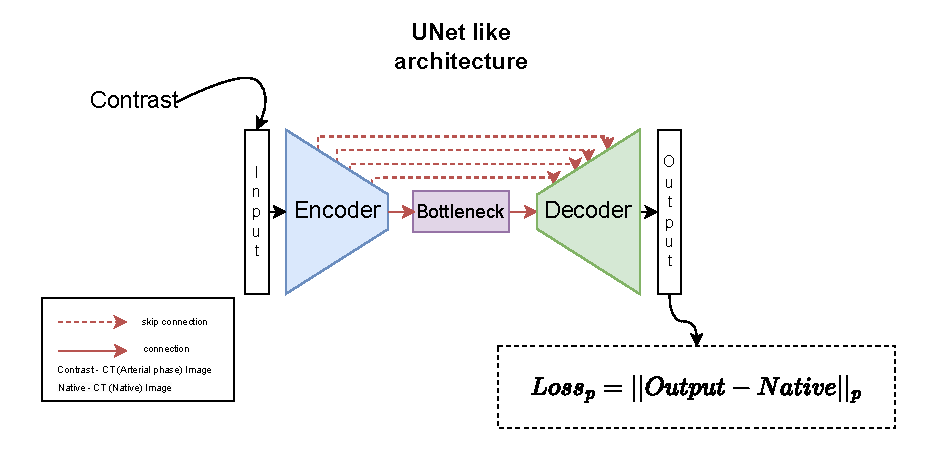
\includegraphics[width=0.8\linewidth]{images/pixel2pixel.pdf}
  \caption{Baseline regression scheme.}
\end{figure}

\subsection{Diffusion}
So if we want to use diffusion for conditional image to image translation, we train a UNet denoiser for the following loss. We will apply DDPM \citep{ho2020denoising} to conditional image-to-image generation. $\pi_{0}$ -- distribution of target images, $\pi_{1}$ -- distribution of conditional images. $\pi_{0} \times \pi_{1}$ -- joint distribution of paired target and conditional images. 
\begin{equation}
    \mathcal{L}_{\text{DDPM}}(\theta) = \mathbb{E}_{\varepsilon \sim \mathcal{N}(0, 1)}\mathbb{E}_{t \sim \mathcal{U}\{0, ..., T\}}\mathbb{E}_{(\mathbf{x}_{0},\mathbf{x}_{1}) \sim \pi_{0} \times \pi_{1}} \left\lVert \varepsilon - \varepsilon_{\theta, t} \left(\alpha(t) \cdot \mathbf{x}_0 + \sigma(t)\cdot \varepsilon, \mathbf{x}_1\right)\right\rVert
    \label{eq:gen_ddpm_loss}
\end{equation}

We have conditions on $\alpha(t)$ and $\sigma(t)$. $\alpha(t), \sigma(t)$ such that $\forall t \in \{0, ..., T\} \xrightarrow{} \alpha(t)^2 + \sigma(t)^2 = 1$. $\mathcal{U} \{0, ..., T\}$ -- is a uniform integer distribution.

If we apply this method in our case, we will get that:
$\pi_{N}$ -- distribution of Native images (target images), $\pi_{C}$ -- distribution of Contrast images (conditional images), $\pi_{N} \times \pi_{C}$ -- joint distribution of paired Native and Contrast images.
So we choose standard linear scheme for $\beta_t$ \citep{ho2020denoising}, using the notation $\alpha_t = 1-\beta_t$ and $\overline{\alpha}_t = \prod\limits_{s=1}^{t}\alpha_s$, so we have $\alpha(t)^2 = \overline{\alpha}_t$,  $\sigma(t)^2 = 1-\overline{\alpha}_t$, $\beta_t = \beta_{start} + (\beta_{end}-\beta{start})\cdot\frac{t}{T}$, where $T, \beta_{start}, \beta_{end}$ -- hyperparameters that are set before training.
\begin{equation}
    \mathcal{L}_{\text{DDPM}}(\theta) = \mathbb{E}_{\varepsilon \sim \mathcal{N}(0, 1)}\mathbb{E}_{t \sim \mathcal{U}\{0, ..., T\}}\mathbb{E}_{(\mathbf{x}_{N},\mathbf{x}_{C}) \sim \pi_{N} \times \pi_{C}} \left\lVert \varepsilon - \varepsilon_{\theta, t} \left(\sqrt{\overline{\alpha}_t} \cdot x_N + \sqrt{1-\overline{\alpha}_t}\cdot \varepsilon, x_C\right)\right\rVert
    \label{eq:ddpm_loss}
\end{equation}

\begin{figure}[h!]
  \centering
  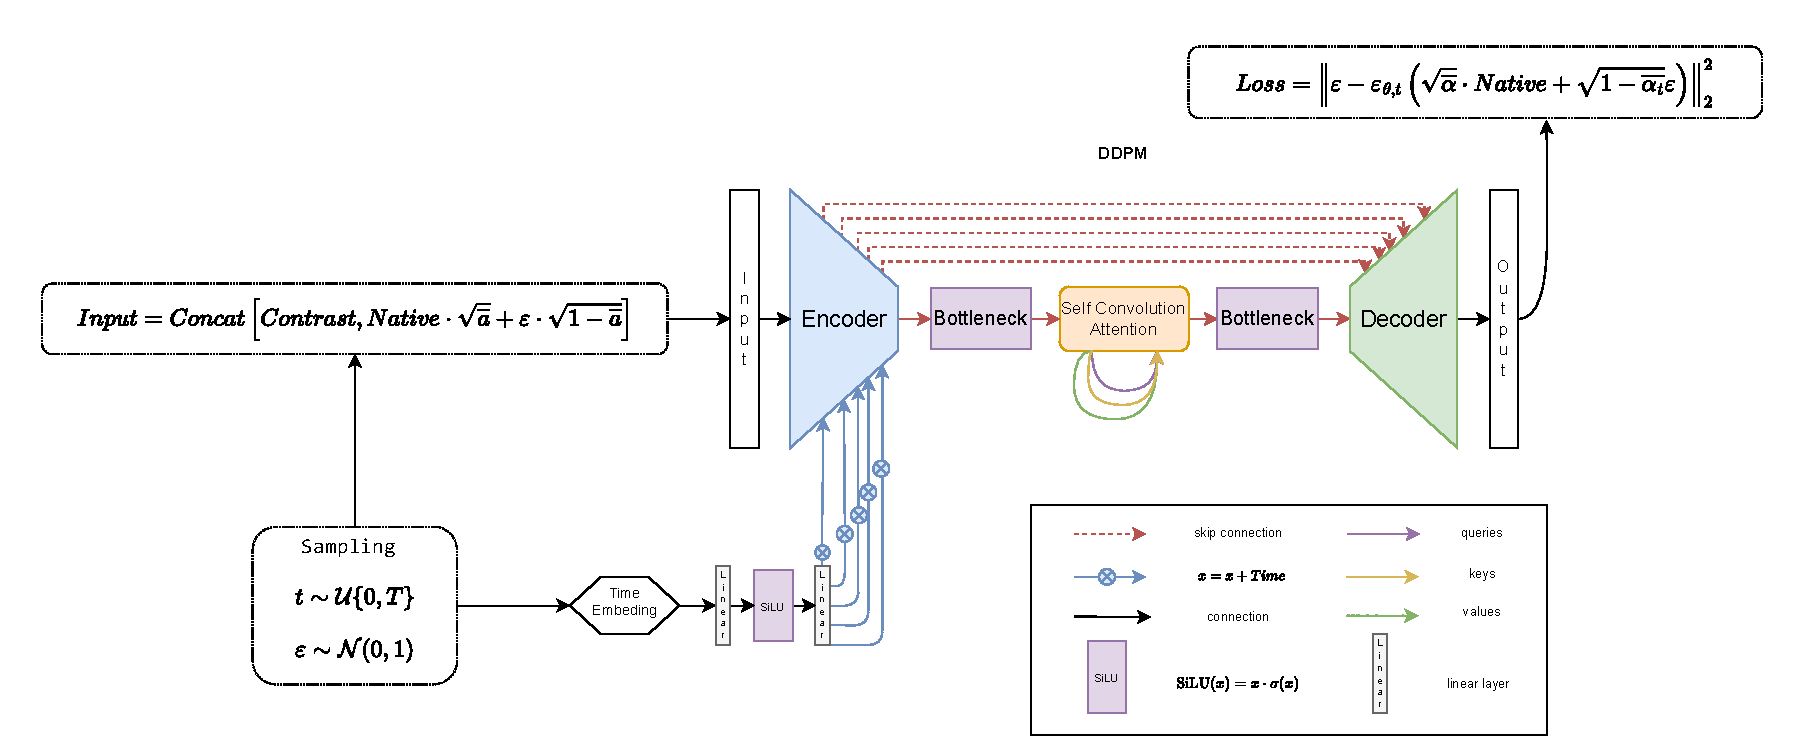
\includegraphics[width=\linewidth]{images/DDPM.pdf}
  \caption{DDPM scheme. Neural network architecture and a visual diagram of training.}
\end{figure}


For sampling we used DDIM-like scheme, to obtain deterministic images from the initial noise.
\begin{equation*}
    \mathbf{x}_{t-1}      =  \sqrt{\frac{1}{1-\beta_t}} \cdot x_t + \left[\sqrt{1-\overline{\alpha}_t} - \sqrt{\frac{1-\overline{\alpha}_{t-1}}{1-\beta_t}} \right] \cdot \varepsilon_\theta\bigl([\mathbf{x}_{\mathrm{img}},\,\mathbf{x}_{t}],\,t\bigr)  
\end{equation*}
%\begin{algorithm}
%\caption{DDIM sampling}
%\begin{algorithmic}[1]
%\State \textbf{Input:}
%noise sample $\mathbf{x}_T\sim\mathcal{N}(0,I)$, conditional image $\mathbf{x}_{\mathrm{img}}$, noise linear scheduler $\{\beta_t\}_{t=1}^T$.
%\State Compute cumulative $\bar\alpha_0 = 1,  \bar\alpha_t = \prod_{s=1}^{t}(1 - \beta_s), \quad t = 1,\dots,T.$
%\For{\(t = T, T-1, \dots, 1\)}
%State Update:
%  \[
%    \mathbf{x}_{t-1}
%      =  \sqrt{\frac{1}{1-\beta_t}} \cdot x_t + \left[\sqrt{1-\overline{\alpha}_t} - \sqrt{\frac{1-\overline{\alpha}_{t-1}}{1-\beta_t}} \right] \cdot \varepsilon_\theta\bigl([\mathbf{x}_{\mathrm{img}},\,\mathbf{x}_{t}],\,t\bigr)
%  \]
%\EndFor
%\State \textbf{Output:} $\mathbf{x}_{0}$.
%\end{algorithmic}
%\end{algorithm}
It is also important to understand that we must use the same noise from which the image will be generated for all axial images of a single patient, otherwise this will lead to a very large heterogeneity in the relative and axial projections.
  
%-------------------------------------------------
\subsection{Flow Matching}
\label{sec:fm_math}
%-------------------------------------------------
Let $\{\pi_{t}\}_{t\in[0,1]}$ be a \emph{probability
path} (\emph{probability path is a continuous trajectory of probability distributions that interpolates between an initial distribution and a target distribution over time.}) that continuously interpolates between an easy‐to‐sample
reference $\pi_{0}$ (e.\,g.\ Gaussian noise) and the data distribution
$\pi_{1}$.
Samples $\mathbf{x}_{t}\!\sim\!\pi_{t}$ evolve according to an ordinary
differential equation (ODE)

\begin{equation}
\frac{\mathrm{d}\mathbf{x}_{t}}{\mathrm{d}t}=f_{\theta}(\mathbf{x}_{t},t),
\qquad
\mathbf{x}_{0}\sim\pi_{0},\;
\mathbf{x}_{1}\sim\pi_{1}.
\label{eq:flow_ode}
\end{equation}

In our case we define $\pi_{0}\!\times\!\pi_{1}$ - as pairs of images of the same patient but from different series, where $\pi_{0}$ - distribution of native images, $\pi_{1}$ - distribution of contrast images.

Define the convex combination $t \in [0, 1]$, $\mathbf{x}_{t}=(1-t)\mathbf{x}_{0}+t\mathbf{x}_{1}$ \label{eq:linear_combination}

and the
\emph{target velocity}
%
\begin{equation}
\mathbf{v}_t
      =\frac{\partial\mathbf{x}_{t}}{\partial t}
      =\mathbf{x}_{1}-\mathbf{x}_{0}.
\label{eq:target_vel}
\end{equation}
%
Flow Matching (FM) trains a neural vector field
$f_{\theta}$ by regressing onto $\mathbf{v}_{t}$
over random $(\mathbf{x}_{0},\mathbf{x}_{1})$ pairs and
$t\!\sim\!\mathcal{U}[0,1]$:
%
\begin{equation}
\mathcal{L}_{\mathrm{FM}}(\theta)=
\mathbb{E}_{t \sim \mathcal{U}[0,1]}\mathbb{E}_{(\mathbf{x}_{0},\mathbf{x}_{1}) \sim \pi_{0} \times \pi_{1}}
\bigl[
\lVert f_{\theta}(\mathbf{x}_{t},t)-
       \mathbf{v}_{t}\rVert_{2}^{2}
\bigr].
\label{eq:fm_loss}
\end{equation}
%
Crucially, Eq.\,\eqref{eq:fm_loss} is \emph{simulation‑free}: no stochastic differential equations need to be solved during training.

Below is a universal diagram of how the model works and learns using the Flow Matching method.

\begin{figure}[h!]
  \centering
  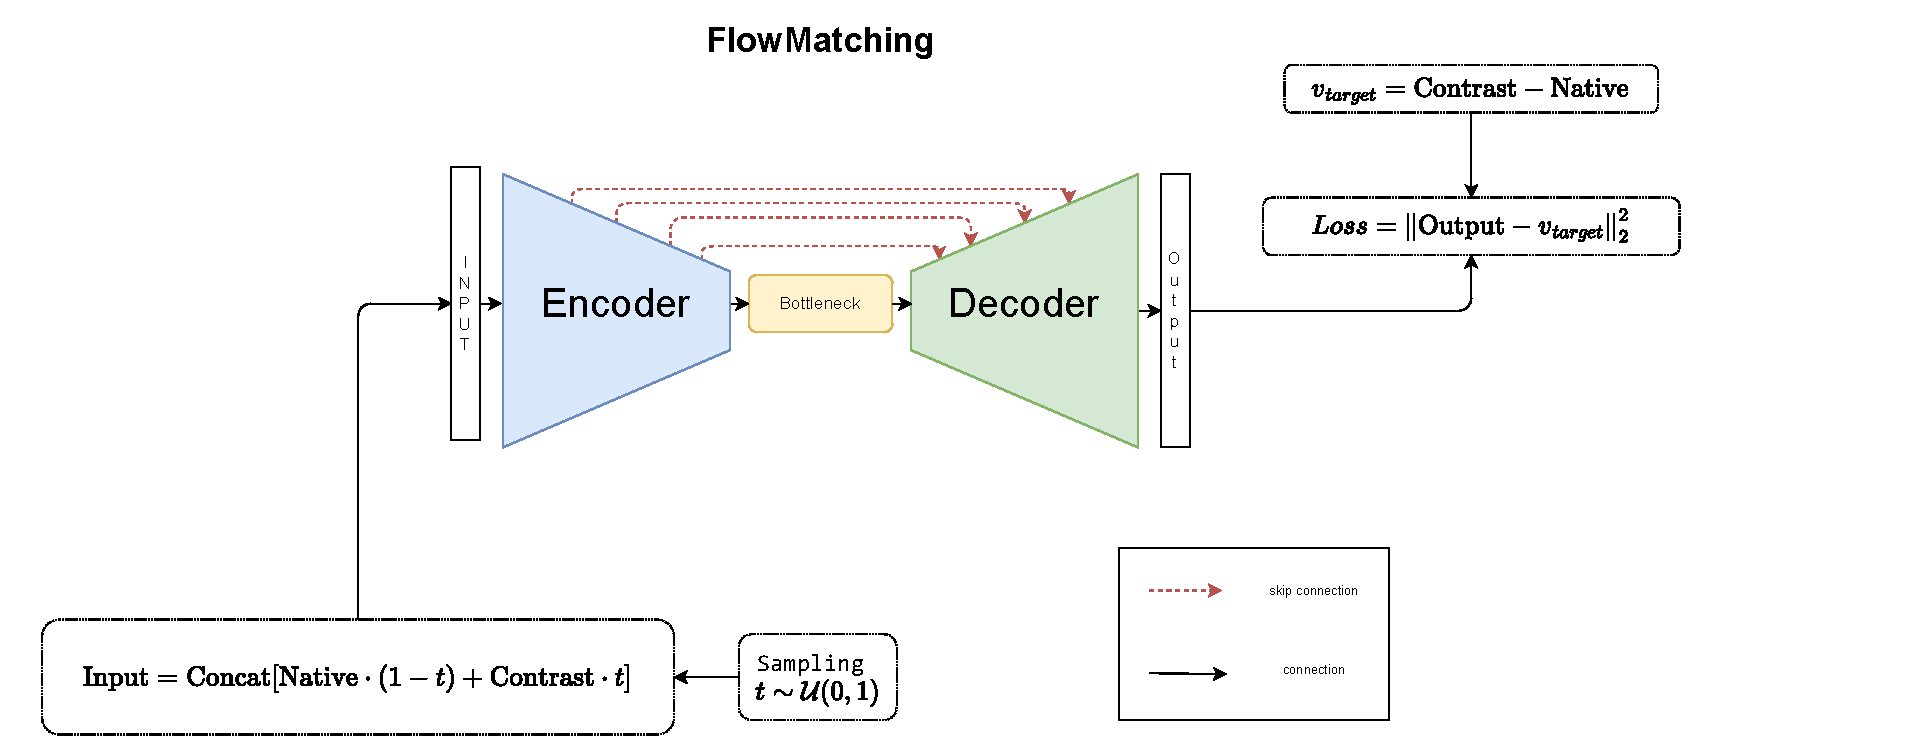
\includegraphics[width=0.7\linewidth]{images/flow.pdf}
  \caption{Flow Matching scheme.}
\end{figure}

We also developed and proposed our own model architecture, TimeResNet.

\begin{figure}[h!]
  \centering
  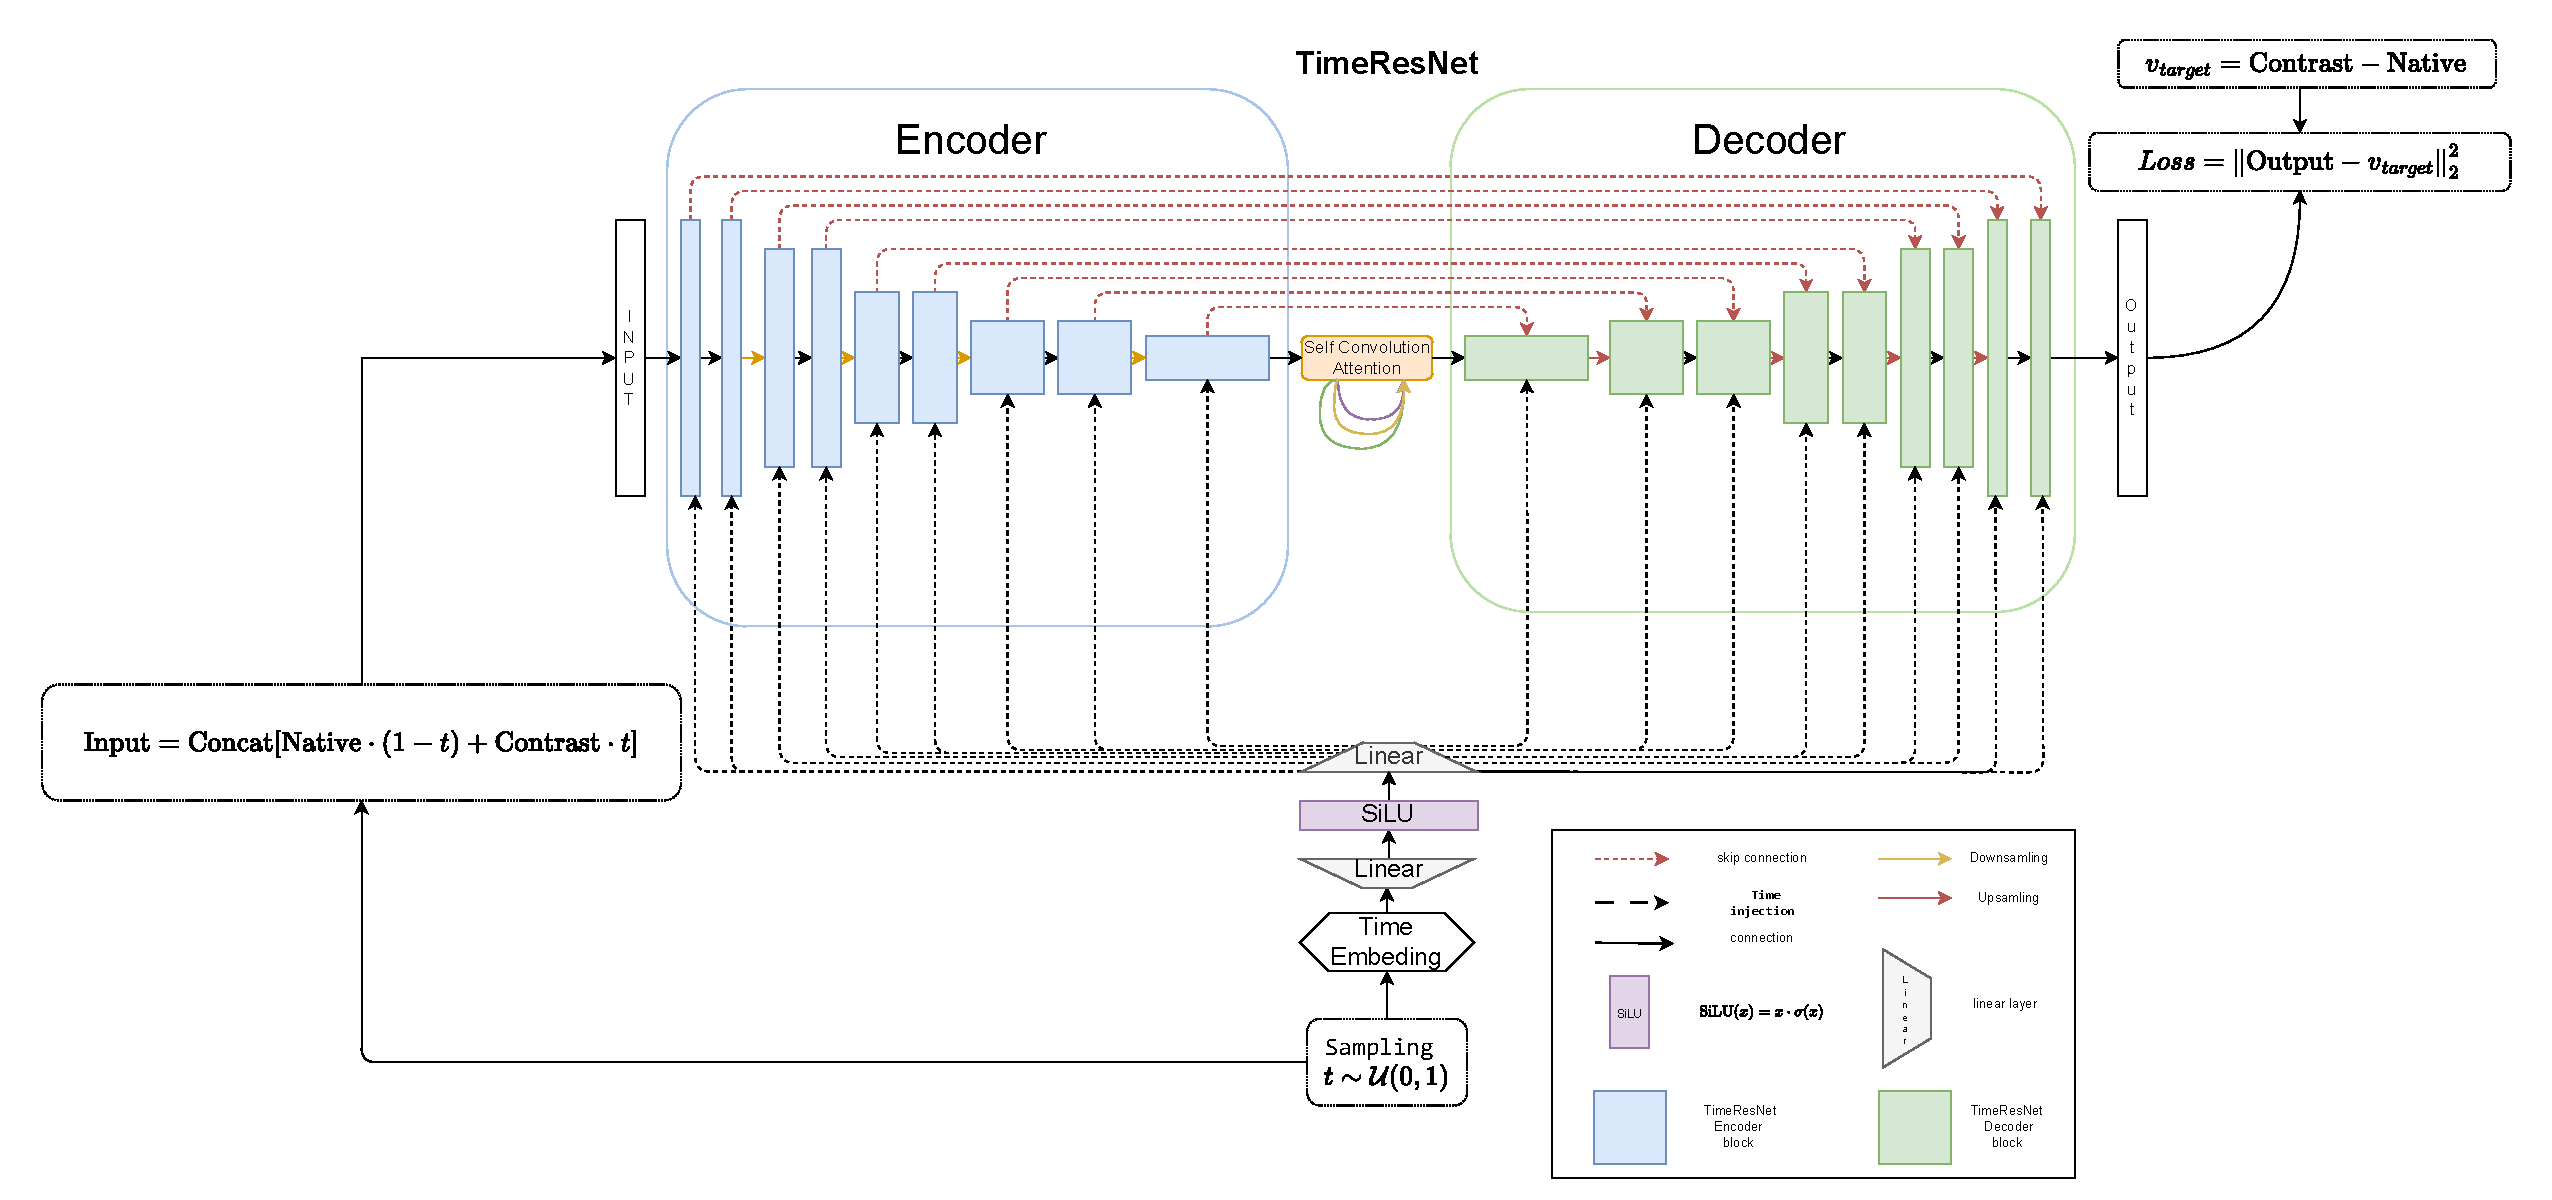
\includegraphics[width=0.95\linewidth]{images/timeresnet.pdf}
  \caption{TimeResNet in Flow Matching scheme.}
\end{figure}

A more detailed description of the Self-Convolution Attention block is given below. We determined that an explicit attention mechanism was necessary to achieve high performance; however, widely adopted architectures such as SwinUNET \citep{cao2022swin} -- which employ a limited, patch-based attention scheme—did not yield substantial gains. Consequently, we elected to insert our attention module between the Bottleneck layers, drawing inspiration from Yang et al. (2019) \citep{yang-etal-2019-convolutional}. To stabilize training, we further incorporated Group Normalization \citep{wu2018group} into the block.

\begin{figure}[h!]
  \centering
  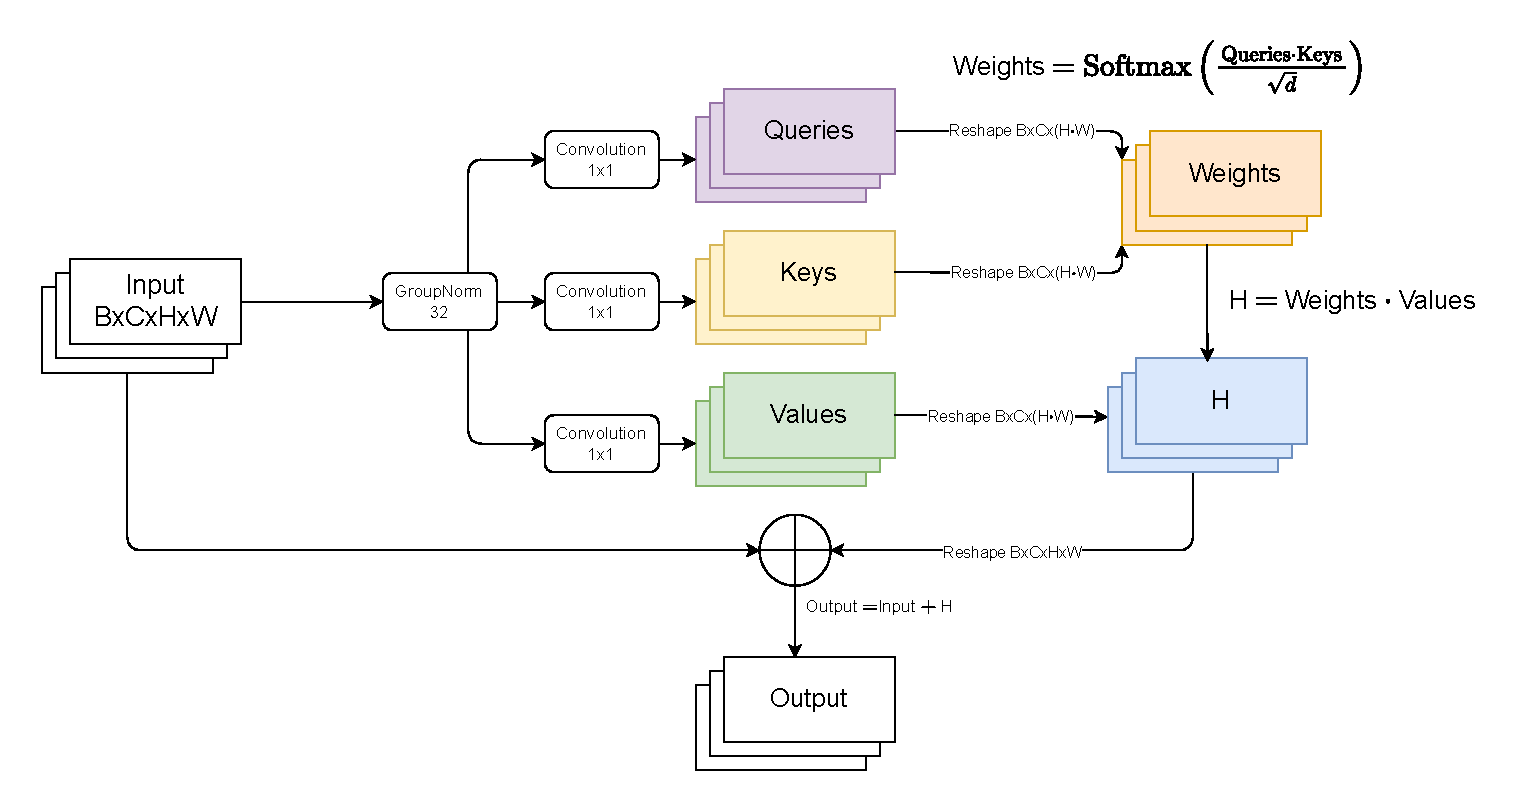
\includegraphics[width=0.85\linewidth]{images/self_attention.pdf}
  \caption{Self convolution attention scheme.}
\end{figure}

After training, sampling reduces to integrating
Eq.\,\eqref{eq:flow_ode} from $t=1$ to $t=0$ with a numerical ODE solver. We have the opportunity to sample both motifs into contrasts and natives from contrasts.


We make full condition on linear combination \eqref{eq:linear_combination} to improve stability of the work and remove stochasticity. To correctly add time intervals to our model, we do the following. We use a standard scheme with sine and cosine embeddings (link to the article), then we feed it into the MLP head, the results of which are fed into each of the ResNet blocks, which initially also uses a linear layer to translate the size to the current number of channels, and then the intermediate values are used as normalization. $h = \textbf{A} \cdot h + \textbf{B}$, where $\textbf{A} \text{ and } \textbf{B}$ are linear and trainable parameters in each block. A more detailed scheme for adding Time embeddings is presented in \ref{app:materials}

%-------------------------------------------------
\section{Experiments}
%-------------------------------------------------
A total of $120$ abdominal CT studies (52561 images) were retrospectively collected, each containing both native and arterial phases (one study per patient), from 3 different CT stations from 3 different hospitals. The dataset was split into $80$ (34992 images) training, $20$ (8197 images) test, and $20$ (9372 images) held‑out patients. Seventy imaging studies were obtained as follows: first, the anatomical region of interest was localized in both the native and contrast‐enhanced series, next, the contrast‐enhanced series were registered to the native series.

All images were taken in the original ($512{\times}512$) shape and clipped to  $[-1000,1000]$ HU before scaling to $[-1, 1]$. As augmentations, we used axis-aligned flips and affine transformations. No intensity‑based perturbations were used in order to preserve Hounsfield integrity.

All models were trained for $30$ epochs with Adam optimizer, batch size was equal $2$. We conducted all the experiments on a node of four NVIDIA RTX 3090 GPU (24 GB). To implement the experiments, we used the PyTorch \citep{paszke2019pytorch} and MONAI framework. 

%-------------------------------------------------
\subsection{Training Dynamics}
%-------------------------------------------------
Detailed model learning trajectory is presented below. We see that the graphs have reached a plateau, but we assume that further scaling in terms of the amount of data, training time, and model size may yield better results, but we tried to use all the resources available to us to present the most valid results in our opinion.

\begin{figure}[h!]
    \centering

    \begin{minipage}[t]{0.48\linewidth}
        \centering
        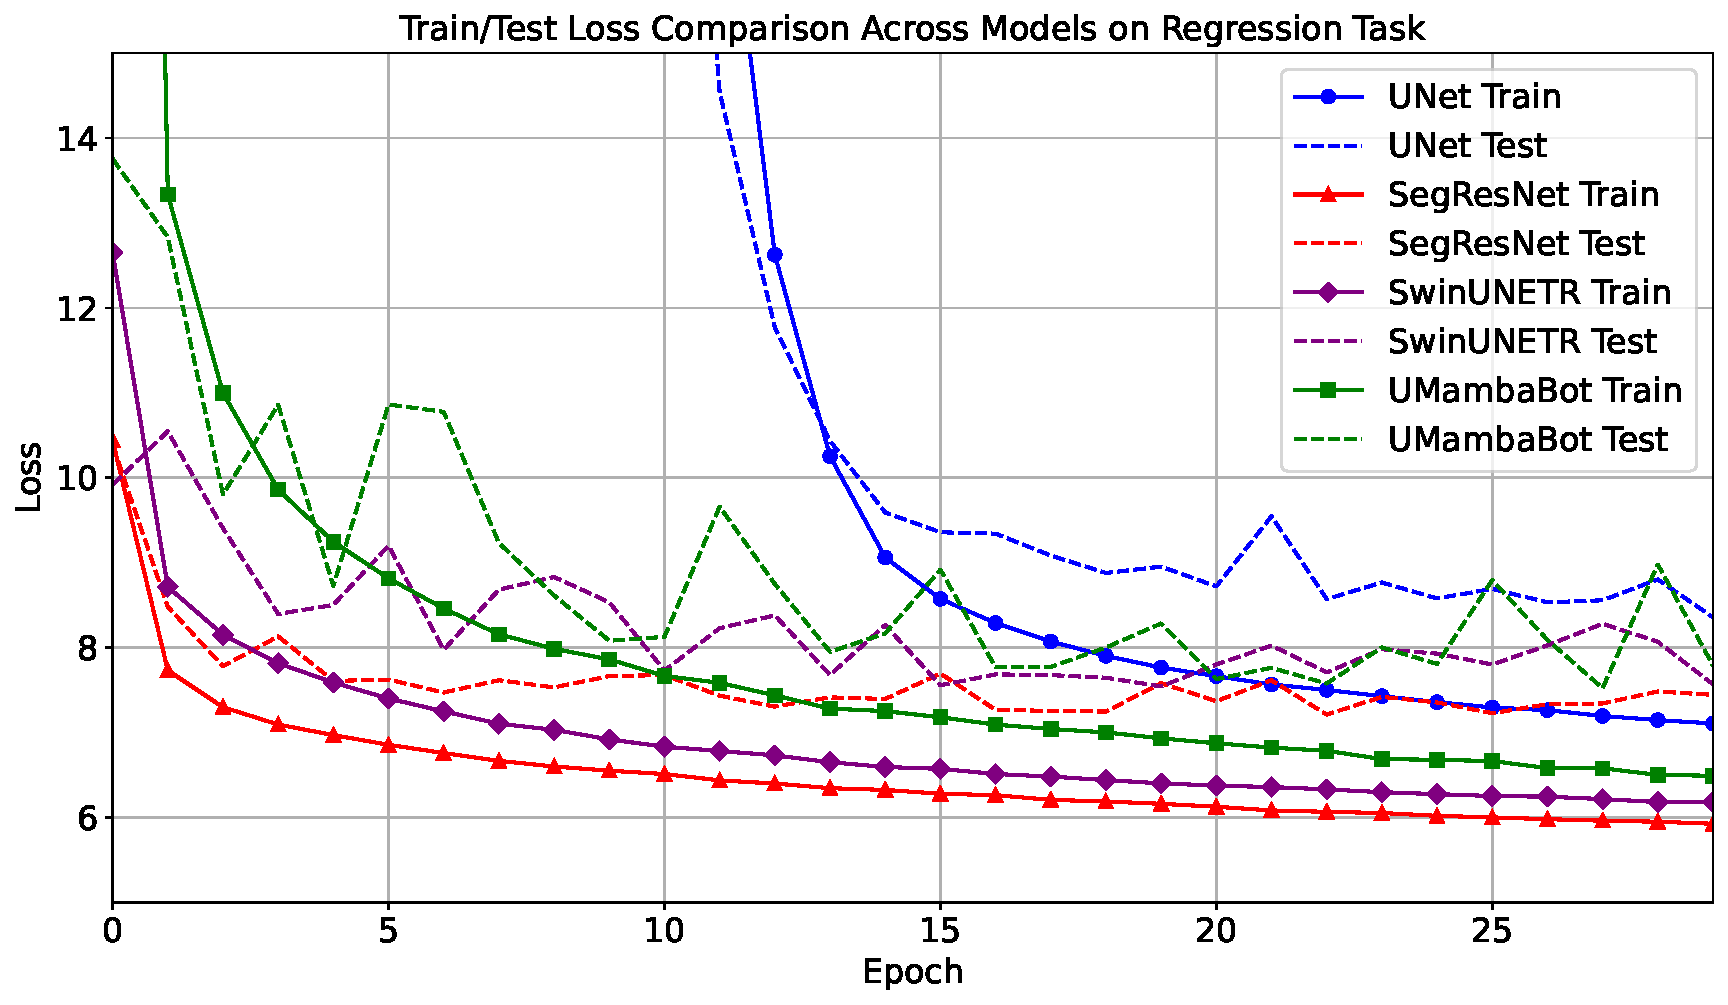
\includegraphics[width=\linewidth]{images/reg_loss_plot.pdf}
        \caption{Dynamics of training different models in the regression task.}
        \label{fig:reg_loss}
    \end{minipage}
    \hfill
    \begin{minipage}[t]{0.48\linewidth}
        \centering
        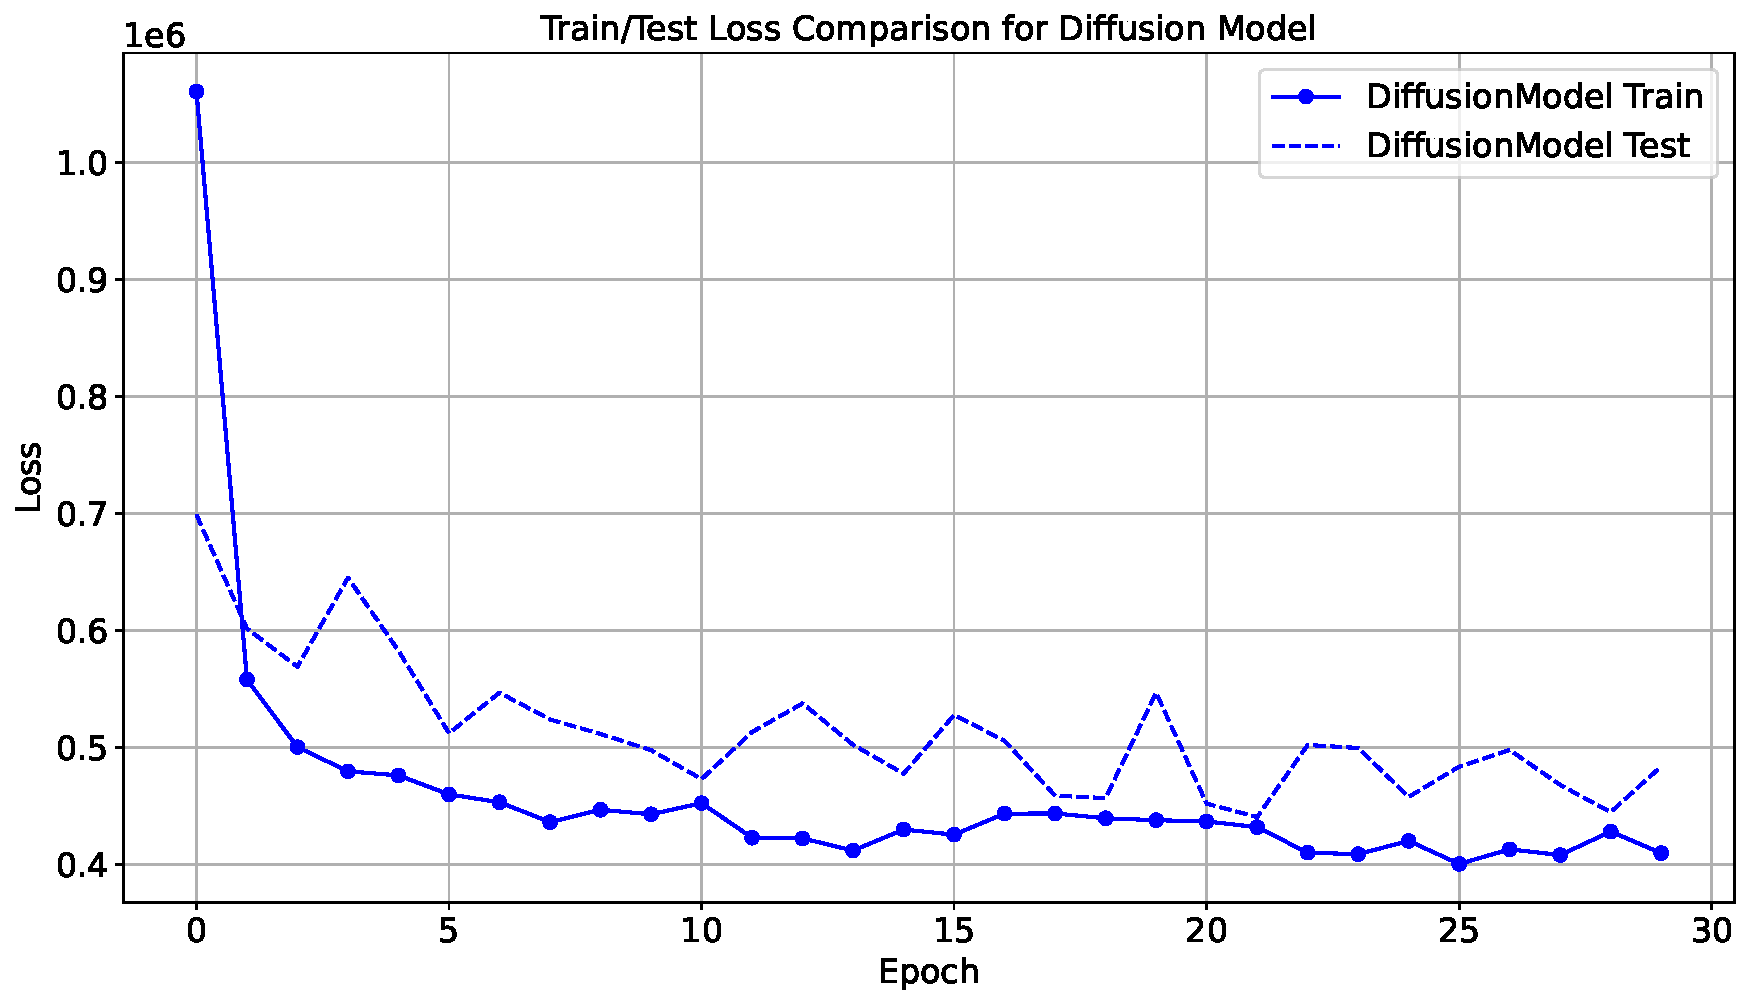
\includegraphics[width=\linewidth]{images/dif_loss_plot.pdf}
        \caption{Dynamics of training model in the diffusion task.}
        \label{fig:dif_loss}
    \end{minipage}

    \vspace{1em}

    \begin{minipage}[t]{0.65\linewidth}
        \centering
        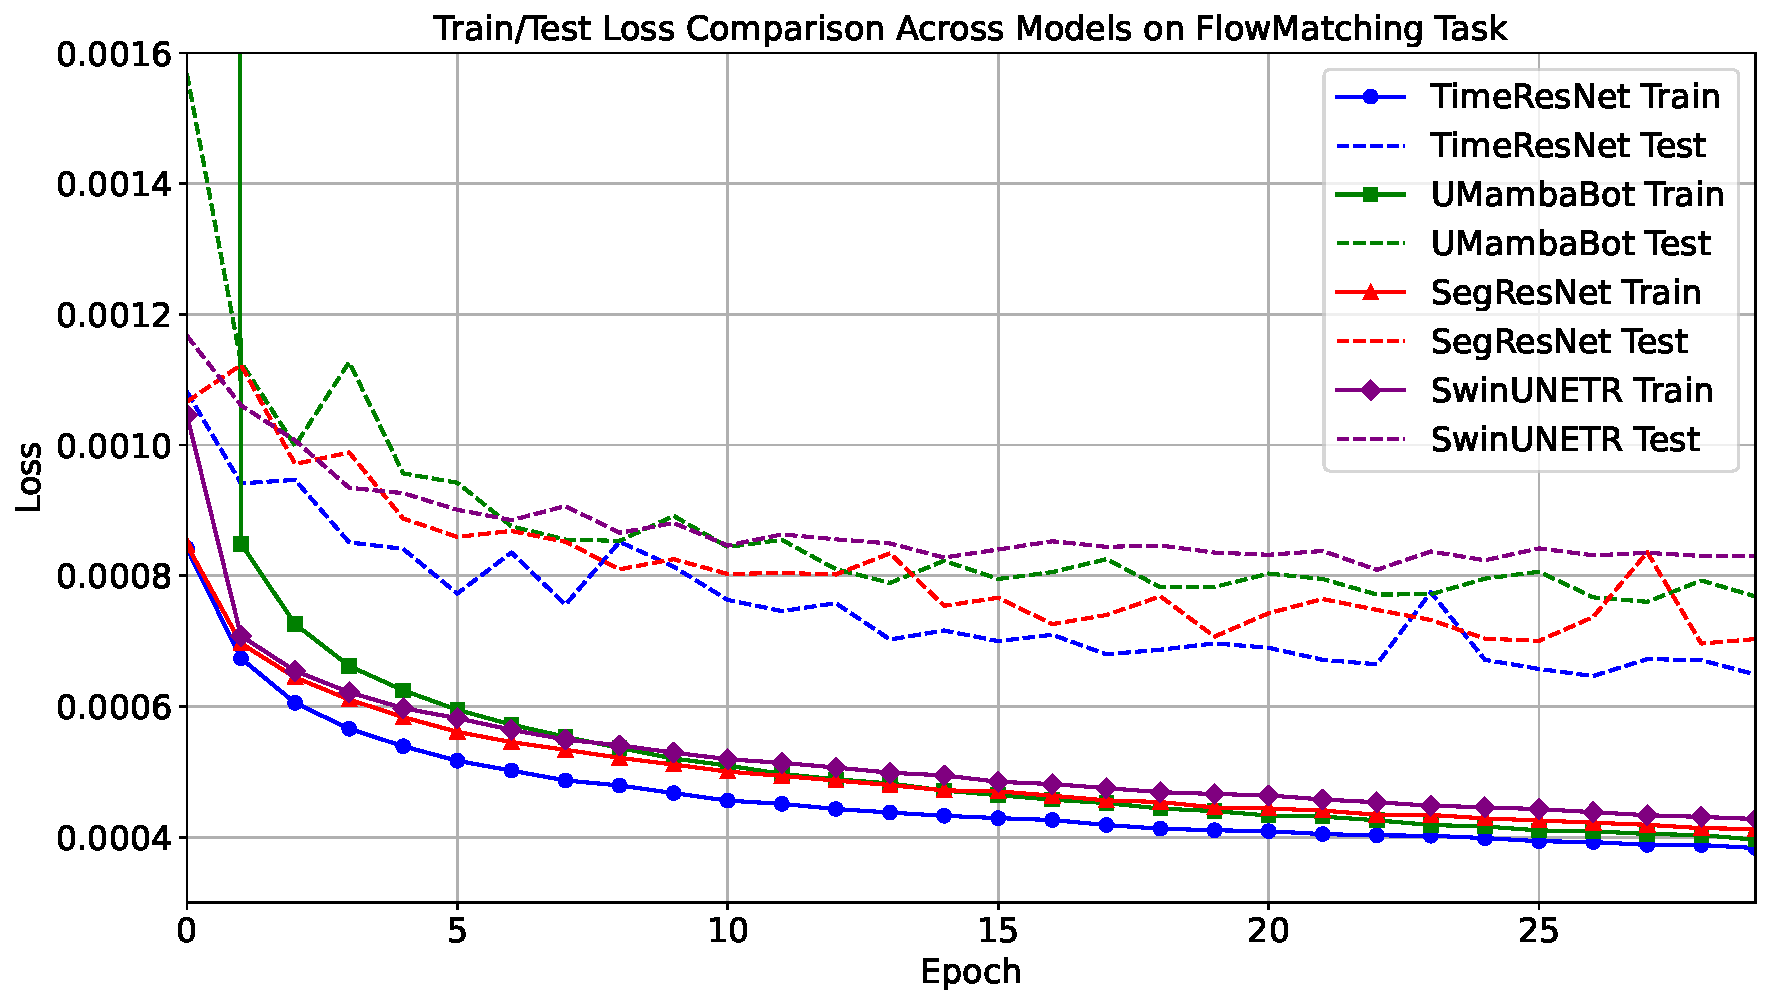
\includegraphics[width=\linewidth]{images/flow_loss_plot.pdf}
        \caption{Dynamics of training different models in the flow matching method.}
        \label{fig:flow_loss}
    \end{minipage}
\end{figure}

We can note that the TimeResNet model we have proposed shows the best convergence compared to the most popular options among CNN, Transformer, and SSM. Umamba architecture needs a certain number of epochs to start showing good results.

%-------------------------------------------------
\subsection{Visual results}
%-------------------------------------------------
In order to evaluate the generation quality of our model in an additional way, we conducted the following experiment. We generated native images from contrast using the SegResNet model for the regression task, generated images using diffusion, and generated images using the TimeResNet model. Then we transferred 20 pairs consisting of a real native and a generated sample to qualified radiologists to blindly determine where the generated image is and where the original one is. Of the 20 examples generated by regression, all 20 examples were correctly classified, and the diffusion examples had the same result. But using the example of our TimeResNet model, the doctor correctly selected 17 cases out of 20. Next, we decided to conduct an experiment where we provide only one image and ask the reader to label it as  a generated or real. We took 20 new cases and generated them in a similar way, so that 10 images were generated and 10 were real. In the same experiment with images generated by diffusion and regression, similar results were obtained and all 20 images were selected correctly. But in the pictures generated using TimeResNet, 14 of the 20 pictures were already correctly selected. It is worth mentioning that our 2 doctors in both experiments used a professional application for viewing medical images - Slicer3D, which allows you to carefully view the image in all 3 projections simultaneously, the doctors performed the screening in the adbomen window. The following conclusions can be drawn from the generated images: in those produced by the regression-based approach, organs such as the kidneys, liver, and aorta are recognizable, but the model tends to blur fine details and smooth out artifacts present in the original CT scans. Diffusion is the easiest to guess due to the fact that the image is unnaturally shifted when viewed in a sagittal projection. But there are difficulties in the pictures obtained using Flow Matching, so with paired studies you can find some details in the liver and kidneys that simply cannot be seen in native images due to the specifics of CT scans. Further improvement of this method can be achieved by improving the quality of the training dataset. You can see from the example that we presented that the difference between a native and contrast image is not only in terms of organs that differ in intensity, but also along the border of the human body. This is due to the fact that the person still moves a little during the CT scan. An example of generation can be found in \ref{app:image_visual}.

\begin{figure}[h!]
    \centering
    \includegraphics[width=0.62\linewidth]{images/small_example.png}
    \caption{Compare different methods and models for translation from Contrast to Native image. The original Contrast and Native are shown below}
    \label{app:image_visual}
\end{figure}

\subsection{Evaluation Metrics}

To evaluate image-to-image translation task we used MAE, although it may not reflect the visual component, but provided that the picture looks visually correct, it is an excellent metric for comparing two models.
\begin{equation}
MAE(x, y) = \frac{1}{H\cdot W}\sum\limits_{i=1}^H\sum\limits_{j=1}^W |x_{ij}-y_{ij}|.
\end{equation}

To balance the MAE we also used the SSIM \citep{1284395}. The SSIM is a commonly used metric for measuring the structural similarity between two images, it is similar to human perception of image quality. It is defined as:
\begin{equation}
SSIM(x, y) = \frac{\mu_x\mu_y+C_1}{\mu_x^2 + \mu_y^2+C_1} \cdot \frac{2\cdot\sigma_{xy}+C_2}{\sigma_x^2 + \sigma_y^2 + C_2},
\label{eq:ssim_loss}
\end{equation}
where $\mu_x, \mu_y$ and $\sigma_x, \sigma_y$ are the means and standard deviations of images x and y respectively, $\sigma_{xy}$ means the covariance of $x$ and $y$. $C_1$ is $(k_1L)^2$ and $C_2$ is $(k_2L)$, where $k_1 = 0.01$, $k_2 = 0.01$ and $L$ is the largest pixel of the image $x$.
Also we used the peak signal-to-noise ratio (PSNR) \citep{korhonen2012peak} to evaluate the similarity between the original image and the generated image. PSNR measures the ratio between the maximum possible value of the original image and the power of distorting noise:
\begin{equation}
\text{PSNR} = 20 \cdot \log_{10}\left( \frac{\text{MAX}(image)}{\sqrt{\text{MSE}}}\right),
\end{equation}
where $\text{MAX}(x)$ denotes the maximum possible pixel value of the image.


%-------------------------------------------------
\subsection{Quantitative Results}
%-------------------------------------------------
All values of the MAE metric are specified for images whose values range from -1000 to 1000 HU, which corresponds to the values of real images. The SSIM values are calculated by translating values from 0 to 1, the PSNR metric is obtained taking into account that the values take values from 0 to 2000, and the maximum value is 2000. All models were compared by translation based on a one-step solution using the Euler method.
\begin{table}[h!]
\centering
\begin{tabular}{lcccccccc}
\toprule
\textbf{Name} 
  & \multicolumn{3}{c}{\textbf{Test}} 
  & \multicolumn{3}{c}{\textbf{Hold-out}} 
  & \textbf{Time} & \textbf{Params}\\
\cmidrule(lr){2-4} \cmidrule(lr){5-7}
   & MAE$\downarrow$ & SSIM$\uparrow$ & PSNR$\uparrow$  
  & MAE$\downarrow$ & SSIM$\uparrow$ & PSNR$\uparrow$ 
  & Seconds$\downarrow$ & Millions $\downarrow$ \\
\midrule
UNet       & 8.132 & 0.976 & 37.629 & 7.051 & 0.979 & 39.220 & \textbf{0.015} & 104.3\\
SegResNet  & \textbf{7.177} & \textbf{0.979} & \textbf{38.103} & \textbf{6.146} & \textbf{0.983} & \textbf{40.108} & \textbf{0.056} & 214.1 \\
SwinUNETR  & 7.465 & 0.978 & 38.046 & 6.485 & \underline{0.982} & 39.865 & 0.087 & 120.1\\
UMambaBot  & \underline{7.220} & \textbf{0.979} & \textbf{38.103} & \underline{6.201} & \underline{0.982} & \underline{39.955} & \underline{0.077} & 141.6\\
\bottomrule
\end{tabular}
\vspace{0.2cm}
\caption{Comparison of neural network regression performance on test and hold-out datasets using MAE, SSIM, PSNR, and inference time in seconds. Best values in \textbf{bold}, second-best values are \underline{underlined}.}
\label{tab:metrics_comparison}
\end{table}

The regression-based method produces good metrics for MAE, but you can see that SSIM is significantly inferior to the FlowMatching method. This loss can also be observed visually, the image is blurred.

\begin{table}[h!]
\centering

\label{tab:ddpm}
\begin{tabular}{lccccc}
\toprule
\textbf{Split} & MAE$\downarrow$ & SSIM $\uparrow$ & PSNR $\uparrow$ & Time (seconds) $\downarrow$\\
\midrule
\textbf{Test}        & 17.822 & 0.935 & 30.192 & 44.2 \\
\textbf{Hold‑out}    & 18.203 & 0.934 & 30.051  & 44.2\\
\bottomrule
\end{tabular}
\vspace{0.2cm}
\caption{Evaluate DDPM performance using MAE, SSIM, and PSNR on test and hold-out datasets.}
\end{table}
The diffusion generation method produces good metrics, but it lags far behind other approaches.


\begin{table}[h!]
\centering
\begin{tabular}{lcccccccc}
\toprule
\textbf{Name} 
  & \multicolumn{3}{c}{\textbf{Test}} 
  & \multicolumn{3}{c}{\textbf{Hold-out}} 
  & \textbf{Time} & \textbf{Params} \\
\cmidrule(lr){2-4} \cmidrule(lr){5-7}
  & MAE$\downarrow$ & SSIM$\uparrow$ & PSNR$\uparrow$  
  & MAE$\downarrow$ & SSIM$\uparrow$ & PSNR$\uparrow$ 
  & Seconds$\downarrow$ & Millions $\downarrow$ \\
\midrule
UMambaBot         & \underline{6.207} & \textbf{0.992} & 38.623 
                  & \textbf{6.171} & \textbf{0.992} & 38.545 & \underline{0.077} & 141.6 \\
SegResNet         & 6.326 & 0.991 & \underline{38.783} 
                  & 6.494 & 0.991 & \underline{38.572} & \textbf{0.056} & 214.1 \\
SwinUNETR         & \textbf{6.235} & \textbf{0.992} & \textbf{38.942} 
                  & \underline{6.229} & \textbf{0.992} & \textbf{38.933} & 0.087 & \textbf{120.1} \\
TimeResNet (Our)   & 6.513 & 0.990 & 38.017 
                  & 6.363 & 0.991 & 38.182 & 0.105 & \underline{124.7} \\
\bottomrule
\end{tabular}
\vspace{0.2cm}
\caption{Comparison of neural network Flow Matching performance (from Contrast to Native) using MAE, SSIM, PSNR, and inference time in seconds on test and hold-out datasets. Best values in \textbf{bold}, second-best values are \underline{underlined}.}
\label{tab:metrics_comparison_contrast}
\end{table}
For the task of translating Contrast to Native, the best metrics are provided by the SwinUNETR architecture. To compare different architectures, we used the simplest method of solving the equation - the one-step Euler method. We conducted a more thorough analysis in terms of selecting a solver and choosing the number of steps, using the TimeResNet example, you can find the results in \ref{app:materials}. Careful selection of the solver leads to a significant improvement in the metrics of our proposed model compared to the values of the architecture metrics in the table.

%-------------------------------------------------
\subsection{Results on subtask segmentation}
%-------------------------------------------------
In order to test the possibility of training real models on our generated images, we conducted the following experiment. We took a hold-out dataset that was not used in training the model, marked the aorta on Native images, and marked the aorta on contrasting images. Next, the contrasting images were converted to native images using the proposed model in the article. We used the nnUNetV2 framework to train the segmentation model. We trained on all 20 images, in order to validate our models, we marked the aorta on an additional 20 native images, on which our models failed.
Dice of the model that was trained on real Native images $= {0.966}$, Dice of the model that was trained on translated Native images $= {0.926}$. These results confirm the huge opportunity for training models on the generated ones, they show metrics comparable with real images.
%-------------------------------------------------
\subsection{Discussion and Limitations}
\label{sec:discussion}
%-------------------------------------------------
Our proposed method and models yield substantial improvements in CT image translation—thereby expanding the available training data and markedly enhancing performance across diverse domains—they also serve effectively as a data-augmentation tool for training robust models capable of operating in dual-domain settings. It is imperative to define the limits of applicability and to caution that radiologists should not draw clinical conclusions based solely on a single series of images synthesized by these models, whether generating contrast-enhanced scans from native data or vice versa. Our future work will focus on addressing challenges associated with extending these techniques to volumetric imaging and on reducing the requisite GPU memory footprint.

%-------------------------------------------------
\section{Conclusion}
%-------------------------------------------------
In this paper, we propose a novel method in medical imaging that allows us to solve two tasks at once, translation from Contrast to Native and translation from Native to Contrast, which reduces the necessary computational resources to train a model for these tasks, and also demonstrates an unprecedented generation rate compared to diffusion models. We offer an architecture that reliably solves these problems and generate stable images. These developments are expected to enhance the potential accessibility of data across diverse modalities for downstream tasks, as well as to support additional augmentation of medical datasets for foundation models.
%-------------------------------------------------
\section{Data availability}
%-------------------------------------------------
Due to confidentiality, data collected for the study are not publicly available for download, however the corresponding authors can be contacted for academic purposes. Tools for deep learning are indicated in the methods
section.

\bibliographystyle{unsrtnat}
\bibliography{references}

\newpage
%-------------------------------------------------
\appendix
The additional material is organized as follows: section A will contain details about metrics and methods of model inference on a test sample, section B will provide details about the selection of hyperparameters in training, section C will provide visual diagrams of training and operation of various parts of the neural network, and section D will provide additional examples of image generation.

\section{Additional quantative results}
%All values of the MAE metric are specified for images whose values range from -1000 to 1000, which corresponds to the values of real images. The SSIM values are calculated by translating values from 0 to 1, the PSNR metric is obtained taking into account that the values take values from 0 to 2000, and the maximum value is 2000.

\subsection{Details}
We measured the ability to convert images with contrast to native images using the models we trained to test their ability to do this. They showed good results. This gives us the opportunity to use the same neural network, but for two types of tasks, it allows us to reduce the time for training two neural networks in the case of UNet Regression, DDPM.
\begin{table}[h!]
\centering
\begin{tabular}{lcccccccc}
\toprule
\textbf{Name} 
  & \multicolumn{3}{c}{\textbf{Test}} 
  & \multicolumn{3}{c}{\textbf{Hold-out}} 
  & \textbf{Time (s)} & \textbf{Params} \\
\cmidrule(lr){2-4} \cmidrule(lr){5-7}
  & MAE$\downarrow$ & SSIM$\uparrow$ & PSNR$\uparrow$  
  & MAE$\downarrow$ & SSIM$\uparrow$ & PSNR$\uparrow$ 
  & Seconds$\downarrow$ & Millions $\downarrow$ \\
\midrule
UMambaBot         & \underline{6.996} & \textbf{0.989} & \underline{39.095} & \underline{6.882} & \underline{0.989} & \underline{38.933} & \underline{0.077} & 141.1 \\
SegResNet         & \textbf{6.431} & \textbf{0.989} & \textbf{39.544} & \textbf{6.426} & \textbf{0.990} & \textbf{39.369} & \textbf{0.056} & 214.1\\
SwinUNETR         & 7.593 & 0.987 & 38.692 & 7.604 & 0.987 & 38.524 & 0.087 & \textbf{120.1} \\
TimeResNet (Our)   & 7.329 & 0.988 & 38.947 & 7.253 & 0.988 & 38.777 & 0.105 & \underline{124.7} \\
\bottomrule
\end{tabular}
\caption{Comparison of neural network Flow Matching performance (from Native to Contrast) using MAE, SSIM, PSNR, and inference time in seconds on test and hold-out datasets. Best values in \textbf{bold}, second-best values are \underline{underlined}.}
\label{tab:flow_metrics_comparison}
\end{table}

In the task of translating from Native to Contrast, the SegResNet architecture wins by a large margin.

\subsection{ODE‑Solver Ablation}
Table~\ref{tab:solver} benchmarks five numerical solvers (Euler \citep{euler1769institutionum}, Midpoint \citep{10.1145/320831.320840}, RK2 \citep{Runge1895}, RK3, RK4 \citep{kutta1901beitrag}, Adams \citep{bashforth1883})
Exponential Integrator) for the best FM model over step budgets $\{1,3,5,10\}$.

We can numerically solve the neural ordinary differential equation using various methods to figure out which method works best and what is the optimal number of steps to choose. With the proper selection of a solver to solve the problem, our model wins by a significant margin over other architectures.

\begin{table}[h!]
\centering
\label{tab:solver}
\begin{tabular}{l ccc ccc cc}
\toprule
\textbf{Solver} 
  & \multicolumn{3}{c}{\textbf{Test}} 
  & \multicolumn{3}{c}{\textbf{Hold-out}} 
  & \textbf{Time} & \textbf{Complexity} \\
\cmidrule(lr){2-4} \cmidrule(lr){5-7} 
  & MAE$\downarrow$ & SSIM$\uparrow$ & PSNR$\uparrow$ 
  & MAE$\downarrow$ & SSIM$\uparrow$ & PSNR$\uparrow$ 
  & Seconds $\downarrow$ & $\downarrow$ \\
\midrule
Euler (1)      & 6.513 & 0.990 & 38.017 & 6.362 & 0.991 & 38.182 & \textbf{0.105} & 1 \\
Euler (2)      & 5.591 & 0.995 & 39.039 & 5.525 & 0.995 & 39.017 & \underline{0.210} & 2 \\
Euler (3)      & \underline{5.529} & \textbf{0.996} & 38.941 & \underline{5.472} & 0.995 & 38.994 & 0.313 & 3 \\
Euler (5)      & 5.565 & 0.995 & 38.899 & 5.526 & 0.995 & 38.951 & 0.521 & 5 \\
RK2   (1)      & \textbf{5.399} & \textbf{0.996} & \textbf{40.017} & \textbf{5.436} & \textbf{0.996} & \textbf{39.776} & 0.209 & 2 \\
RK3   (1)      & 5.553 & 0.995 & 39.193 & 5.553 & 0.995 & 39.122 & 0.313 & 3 \\
RK4   (1)      & 5.674 & 0.995 & \underline{39.408} & 5.716 & 0.995 & \underline{39.257} & 0.419 & 4 \\
Mid Point (1)  & 5.601 & 0.995 & 39.106 & 5.611 & 0.995 & 39.047 & \underline{0.210} & 2 \\
Mid Point (3)  & 5.744 & 0.995 & 38.882 & 5.759 & 0.995 & 38.923 & 0.628 & 6 \\
\bottomrule
\end{tabular}
\caption{Comparison of different solvers (from Contrast to Native) for TimeResNet (our) using MAE, SSIM, PSNR, and inference time in seconds on test and hold-out datasets. Best values in \textbf{bold}, second-best values are \underline{underlined}.}
\end{table}

By complexity here, we mean the number of calls to the neural network to calculate the gradient when generating a single image.

\section{Additional implementation details}
\label{app:materials}

\subsection{2D Processing Justification}
Due to the limited computing resources available, we decided to solve this problem in 2D, since 3D requires much more computing resources and a lot of data, but a full-fledged volume does not fit on one GPU, so it would require a latent‐space solution, which still demands significant resources. Moreover, clinicians typically review studies in the axial plane (though not always), making 2D axial slices a natural choice. We therefore restrict our method to 2D axial processing.

\subsection{Image Preprocessing and Resizing}
When down‐sampling inputs, one can either resample to a uniform spacing or to a fixed pixel size. We chose a fixed image size of \(512\times512\), since nearly all DICOM slices in our dataset already conform to this dimension. Avoiding on‐the‐fly resizing during inference eliminates an extra source of error. Additionally, variations in original spacing act as implicit data augmentation, improving model robustness. We acknowledge that 2D methods may lack inter‐slice context and can yield inconsistent predictions across different planes (e.g., axial vs.\ sagittal), as seen in diffusion experiments; however, our approach demonstrates stable and consistent contrast‐to‐native predictions slice‐by‐slice within the same study.

\subsection{Data Normalization and Clipping}
To harmonize input intensities across scanners, we clip CT Hounsfield Units to \([-1000, 1000]\), then linearly rescale to \([-1,1]\). This range covers the vast majority of soft‐tissue contrasts while ensuring numerical stability during training.

\subsection{Data Augmentation and Optimization}
We apply geometric augmentations via the MONAI framework:
\begin{itemize}
  \item Random flips along \(x\) and \(y\) axes (50\% each),
  \item Random 90° rotations (up to 3 turns, 50\% probability),
  \item Random affine transforms (70\% probability) with: rotation up to \(\pm45^\circ\), translation up to \(\pm102.4\) pixels, shear up to \(\pm10^\circ\).
\end{itemize}

We train using Adam with hyperparameters: $
  \text{learning rate}=2\cdot10^{-5},\quad
  \text{weight decay}=0,\quad
  \beta_1=0.9,\quad
  \beta_2=0.999.$ Batch size was 2.

\subsection{Training Data Selection and Dual‐Energy Exclusion}
To minimize misregistration due to patient motion between acquisitions, we remove series where we have different origins and spacing between two series. Although dual‐energy CT could in principle provide “native” images directly, such data are scarce, and the vendor‐reconstructed “native” series result from proprietary algorithms that may not faithfully represent true tissue contrast. Therefore, we exclude dual‐energy studies to ensure the network learns genuine native-to-contrast mappings.

\subsection{Image Registration}
In order to improve the quality and purity of the data, we registered images with contrast to native images. We employ the ANTs library with the “deformable SyN only” transform, providing a body‐mask to focus optimization on the anatomy. This configuration yielded the best mean absolute error (MAE) and mutual information (MI) improvements, and was faster than alternative ANTs transforms.


%-------------------------------------------------
\section{Additional visual results and discussion}
%-------------------------------------------------
The generation examples are presented in 3 projections, and each of the projections shows the difference between the original native image. The picture was clipped into the abdominal window for a clearer understanding of the difference, since in other windows or without an image clip at all, the difference is much less noticeable, and we are primarily interested in the abdominal window.
\begin{figure}[h!]
    \centering
    \includegraphics[width=0.75\linewidth]{images/projection_montage.png}
    \caption{Compare different methods and models for translation from Contrast to Native image. The original Contrast and Native are shown below}
    \label{app:image_visual}
\end{figure}

%-------------------------------------------------
\newpage
\section{Architecture details}
\subsection{Time embedding mechanism}
One nontrivial challenge is how to encode temporal information so that the model fully captures context and can accurately predict the vector field between two images at a given time point. We evaluated several strategies and found the following approach to be most effective, yielding substantial performance gains. Because the model tends to “forget” the temporal signal, we inject temporal embeddings into every block of the encoder. In addition, we introduce a lightweight linear projection layer in each block, enabling it to learn the specific dependencies it requires without unduly increasing the overall parameter count. This linear layer operates analogously to an instance‐normalization layer, allowing independent modulation of each channel’s activations. The temporal embeddings themselves are constructed using the sinusoidal scheme described in \citep{vaswani2017attention}. To capture nonlinear temporal interactions, we further process these sinusoidal embeddings through a small multilayer perceptron, and the resulting feature vector is added to the input of each ResNet block. 
In the schematic below $A, B$ denote trainable vectors of length $C$, which are applied element‐wise to the output of the SiLU activation. For convenience, one linear layer of length $2\cdot C$ is trained, which is then divided into two vectors -- A, B. 
If the output of the nonlinear layer,  h, has dimensions $(B$ x $C$ x $H$ x $W)$, then the resulting tensor likewise has dimensions $(B$ x $C$ x $H$ x $W)$, with the multiplication broadcast along the channel dimension.

\begin{figure}[h!]
  \centering
  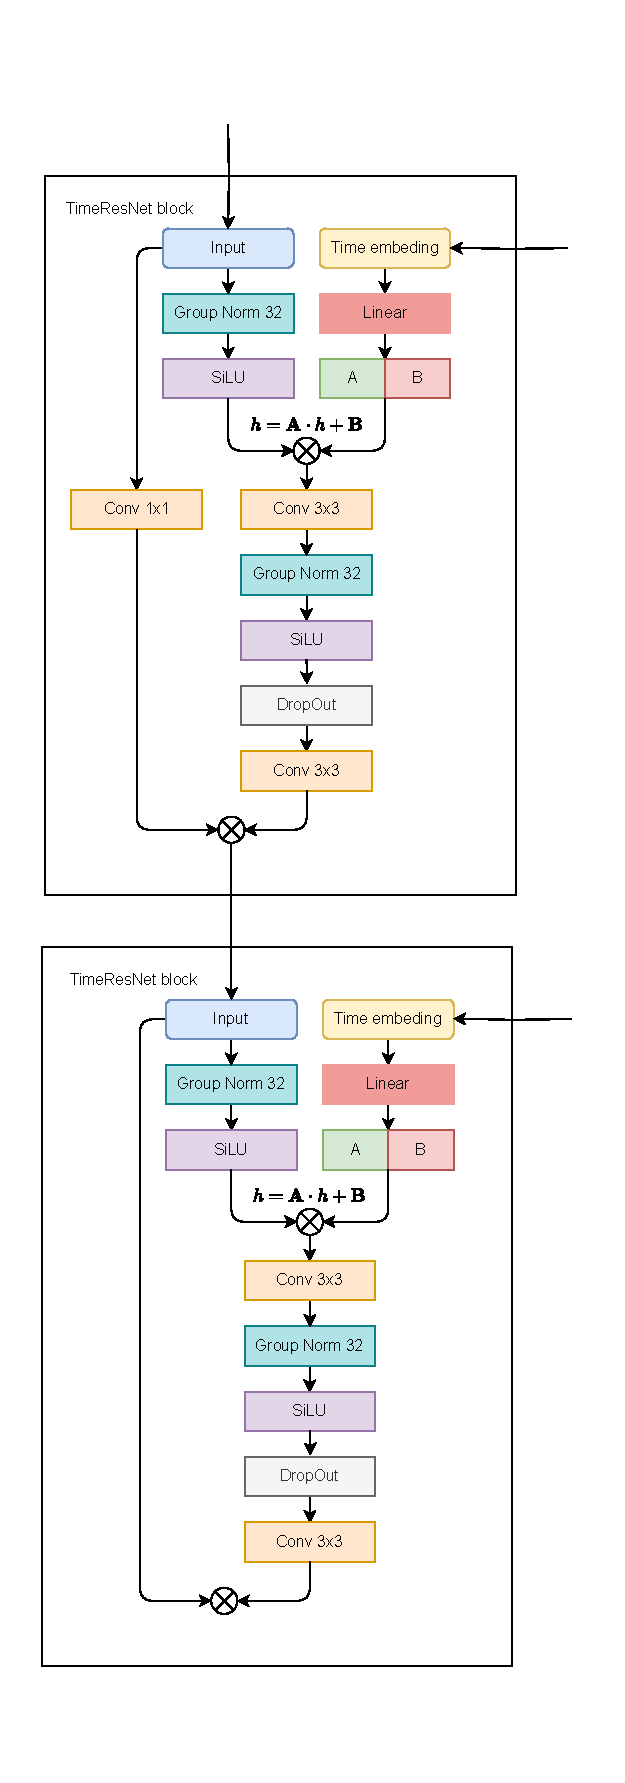
\includegraphics[height=0.5\paperheight]{images/Embeding.pdf}
  \caption{Time embedding mechanism.}
\end{figure}



\newpage

%%%%%%%%%%%%%%%%%%%%%%%%%%%%%%%%%%%%%%%%%%%%%%%%%%%%%%%%%%%%

\newpage
\section*{NeurIPS Paper Checklist}
\if 0
%%% BEGIN INSTRUCTIONS %%%
The checklist is designed to encourage best practices for responsible machine learning research, addressing issues of reproducibility, transparency, research ethics, and societal impact. Do not remove the checklist: {\bf The papers not including the checklist will be desk rejected.} The checklist should follow the references and follow the (optional) supplemental material.  The checklist does NOT count towards the page
limit. 

Please read the checklist guidelines carefully for information on how to answer these questions. For each question in the checklist:
\begin{itemize}
    \item You should answer \answerYes{}, \answerNo{}, or \answerNA{}.
    \item \answerNA{} means either that the question is Not Applicable for that particular paper or the relevant information is Not Available.
    \item Please provide a short (1–2 sentence) justification right after your answer (even for NA). 
   % \item {\bf The papers not including the checklist will be desk rejected.}
\end{itemize}

{\bf The checklist answers are an integral part of your paper submission.} They are visible to the reviewers, area chairs, senior area chairs, and ethics reviewers. You will be asked to also include it (after eventual revisions) with the final version of your paper, and its final version will be published with the paper.

The reviewers of your paper will be asked to use the checklist as one of the factors in their evaluation. While "\answerYes{}" is generally preferable to "\answerNo{}", it is perfectly acceptable to answer "\answerNo{}" provided a proper justification is given (e.g., "error bars are not reported because it would be too computationally expensive" or "we were unable to find the license for the dataset we used"). In general, answering "\answerNo{}" or "\answerNA{}" is not grounds for rejection. While the questions are phrased in a binary way, we acknowledge that the true answer is often more nuanced, so please just use your best judgment and write a justification to elaborate. All supporting evidence can appear either in the main paper or the supplemental material, provided in appendix. If you answer \answerYes{} to a question, in the justification please point to the section(s) where related material for the question can be found.

IMPORTANT, please:
\begin{itemize}
    \item {\bf Delete this instruction block, but keep the section heading ``NeurIPS paper checklist"},
    \item  {\bf Keep the checklist subsection headings, questions/answers and guidelines below.}
    \item {\bf Do not modify the questions and only use the provided macros for your answers}.
\end{itemize} 
 

%%% END INSTRUCTIONS %%%
\fi

\begin{enumerate}

\item {\bf Claims}
    \item[] Question: Do the main claims made in the abstract and introduction accurately reflect the paper's contributions and scope?
    \item[] Answer: \answerYes{} % Replace by \answerYes{}, \answerNo{}, or \answerNA{}.
    \item[] Justification: The main claims made in the abstract and introduction accurately reflect the paper’s contributions and scope.
    \item[] Guidelines:
    \begin{itemize}
        \item The answer NA means that the abstract and introduction do not include the claims made in the paper.
        \item The abstract and/or introduction should clearly state the claims made, including the contributions made in the paper and important assumptions and limitations. A No or NA answer to this question will not be perceived well by the reviewers. 
        \item The claims made should match theoretical and experimental results, and reflect how much the results can be expected to generalize to other settings. 
        \item It is fine to include aspirational goals as motivation as long as it is clear that these goals are not attained by the paper. 
    \end{itemize}

\item {\bf Limitations}
    \item[] Question: Does the paper discuss the limitations of the work performed by the authors?
    \item[] Answer: \answerYes{} % Replace by \answerYes{}, \answerNo{}, or \answerNA{}.
    \item[] Justification: We have discussed the limitations of the work in Section \ref{sec:discussion}
    \item[] Guidelines:
    \begin{itemize}
        \item The answer NA means that the paper has no limitation while the answer No means that the paper has limitations, but those are not discussed in the paper. 
        \item The authors are encouraged to create a separate "Limitations" section in their paper.
        \item The paper should point out any strong assumptions and how robust the results are to violations of these assumptions (e.g., independence assumptions, noiseless settings, model well-specification, asymptotic approximations only holding locally). The authors should reflect on how these assumptions might be violated in practice and what the implications would be.
        \item The authors should reflect on the scope of the claims made, e.g., if the approach was only tested on a few datasets or with a few runs. In general, empirical results often depend on implicit assumptions, which should be articulated.
        \item The authors should reflect on the factors that influence the performance of the approach. For example, a facial recognition algorithm may perform poorly when image resolution is low or images are taken in low lighting. Or a speech-to-text system might not be used reliably to provide closed captions for online lectures because it fails to handle technical jargon.
        \item The authors should discuss the computational efficiency of the proposed algorithms and how they scale with dataset size.
        \item If applicable, the authors should discuss possible limitations of their approach to address problems of privacy and fairness.
        \item While the authors might fear that complete honesty about limitations might be used by reviewers as grounds for rejection, a worse outcome might be that reviewers discover limitations that aren't acknowledged in the paper. The authors should use their best judgment and recognize that individual actions in favor of transparency play an important role in developing norms that preserve the integrity of the community. Reviewers will be specifically instructed to not penalize honesty concerning limitations.
    \end{itemize}

\item {\bf Theory Assumptions and Proofs}
    \item[] Question: For each theoretical result, does the paper provide the full set of assumptions and a complete (and correct) proof?
    \item[] Answer: \answerNA{} % Replace by \answerYes{}, \answerNo{}, or \answerNA{}.
    \item[] Justification: The paper does not include theoretical results.
    \item[] Guidelines:
    \begin{itemize}
        \item The answer NA means that the paper does not include theoretical results. 
        \item All the theorems, formulas, and proofs in the paper should be numbered and cross-referenced.
        \item All assumptions should be clearly stated or referenced in the statement of any theorems.
        \item The proofs can either appear in the main paper or the supplemental material, but if they appear in the supplemental material, the authors are encouraged to provide a short proof sketch to provide intuition. 
        \item Inversely, any informal proof provided in the core of the paper should be complemented by formal proofs provided in appendix or supplemental material.
        \item Theorems and Lemmas that the proof relies upon should be properly referenced. 
    \end{itemize}

    \item {\bf Experimental Result Reproducibility}
    \item[] Question: Does the paper fully disclose all the information needed to reproduce the main experimental results of the paper to the extent that it affects the main claims and/or conclusions of the paper (regardless of whether the code and data are provided or not)?
    \item[] Answer: \answerYes{} % Replace by \answerYes{}, \answerNo{}, or \answerNA{}.
    \item[] Justification: All details of the proposed method are included in the paper.
    \item[] Guidelines:
    \begin{itemize}
        \item The answer NA means that the paper does not include experiments.
        \item If the paper includes experiments, a No answer to this question will not be perceived well by the reviewers: Making the paper reproducible is important, regardless of whether the code and data are provided or not.
        \item If the contribution is a dataset and/or model, the authors should describe the steps taken to make their results reproducible or verifiable. 
        \item Depending on the contribution, reproducibility can be accomplished in various ways. For example, if the contribution is a novel architecture, describing the architecture fully might suffice, or if the contribution is a specific model and empirical evaluation, it may be necessary to either make it possible for others to replicate the model with the same dataset, or provide access to the model. In general. releasing code and data is often one good way to accomplish this, but reproducibility can also be provided via detailed instructions for how to replicate the results, access to a hosted model (e.g., in the case of a large language model), releasing of a model checkpoint, or other means that are appropriate to the research performed.
        \item While NeurIPS does not require releasing code, the conference does require all submissions to provide some reasonable avenue for reproducibility, which may depend on the nature of the contribution. For example
        \begin{enumerate}
            \item If the contribution is primarily a new algorithm, the paper should make it clear how to reproduce that algorithm.
            \item If the contribution is primarily a new model architecture, the paper should describe the architecture clearly and fully.
            \item If the contribution is a new model (e.g., a large language model), then there should either be a way to access this model for reproducing the results or a way to reproduce the model (e.g., with an open-source dataset or instructions for how to construct the dataset).
            \item We recognize that reproducibility may be tricky in some cases, in which case authors are welcome to describe the particular way they provide for reproducibility. In the case of closed-source models, it may be that access to the model is limited in some way (e.g., to registered users), but it should be possible for other researchers to have some path to reproducing or verifying the results.
        \end{enumerate}
    \end{itemize}


\item {\bf Open access to data and code}
    \item[] Question: Does the paper provide open access to the data and code, with sufficient instructions to faithfully reproduce the main experimental results, as described in supplemental material?
    \item[] Answer: \answerYes{} % Replace by \answerYes{}, \answerNo{}, or \answerNA{}.
    \item[] Justification:  All the code and model weights will be released upon paper acceptance, data will be available on request.
    \item[] Guidelines:
    \begin{itemize}
        \item The answer NA means that paper does not include experiments requiring code.
        \item Please see the NeurIPS code and data submission guidelines (\url{https://nips.cc/public/guides/CodeSubmissionPolicy}) for more details.
        \item While we encourage the release of code and data, we understand that this might not be possible, so “No” is an acceptable answer. Papers cannot be rejected simply for not including code, unless this is central to the contribution (e.g., for a new open-source benchmark).
        \item The instructions should contain the exact command and environment needed to run to reproduce the results. See the NeurIPS code and data submission guidelines (\url{https://nips.cc/public/guides/CodeSubmissionPolicy}) for more details.
        \item The authors should provide instructions on data access and preparation, including how to access the raw data, preprocessed data, intermediate data, and generated data, etc.
        \item The authors should provide scripts to reproduce all experimental results for the new proposed method and baselines. If only a subset of experiments are reproducible, they should state which ones are omitted from the script and why.
        \item At submission time, to preserve anonymity, the authors should release anonymized versions (if applicable).
        \item Providing as much information as possible in supplemental material (appended to the paper) is recommended, but including URLs to data and code is permitted.
    \end{itemize}


\item {\bf Experimental Setting/Details}
    \item[] Question: Does the paper specify all the training and test details (e.g., data splits, hyperparameters, how they were chosen, type of optimizer, etc.) necessary to understand the results?
    \item[] Answer: \answerYes{} % Replace by \answerYes{}, \answerNo{}, or \answerNA{}.
    \item[] Justification: All details included in the paper.
    \item[] Guidelines:
    \begin{itemize}
        \item The answer NA means that the paper does not include experiments.
        \item The experimental setting should be presented in the core of the paper to a level of detail that is necessary to appreciate the results and make sense of them.
        \item The full details can be provided either with the code, in appendix, or as supplemental material.
    \end{itemize}

\item {\bf Experiment Statistical Significance}
    \item[] Question: Does the paper report error bars suitably and correctly defined or other appropriate information about the statistical significance of the experiments?
    \item[] Answer: \answerNo{} % Replace by \answerYes{}, \answerNo{}, or \answerNA{}.
    \item[] Justification: NA
    \item[] Guidelines:
    \begin{itemize}
        \item The answer NA means that the paper does not include experiments.
        \item The authors should answer "Yes" if the results are accompanied by error bars, confidence intervals, or statistical significance tests, at least for the experiments that support the main claims of the paper.
        \item The factors of variability that the error bars are capturing should be clearly stated (for example, train/test split, initialization, random drawing of some parameter, or overall run with given experimental conditions).
        \item The method for calculating the error bars should be explained (closed form formula, call to a library function, bootstrap, etc.)
        \item The assumptions made should be given (e.g., Normally distributed errors).
        \item It should be clear whether the error bar is the standard deviation or the standard error of the mean.
        \item It is OK to report 1-sigma error bars, but one should state it. The authors should preferably report a 2-sigma error bar than state that they have a 96\% CI, if the hypothesis of Normality of errors is not verified.
        \item For asymmetric distributions, the authors should be careful not to show in tables or figures symmetric error bars that would yield results that are out of range (e.g. negative error rates).
        \item If error bars are reported in tables or plots, The authors should explain in the text how they were calculated and reference the corresponding figures or tables in the text.
    \end{itemize}

\item {\bf Experiments Compute Resources}
    \item[] Question: For each experiment, does the paper provide sufficient information on the computer resources (type of compute workers, memory, time of execution) needed to reproduce the experiments?
    \item[] Answer: \answerYes{} % Replace by \answerYes{}, \answerNo{}, or \answerNA{}.
    \item[] Justification: All the experiments are conducted on 4 RTX 3090 24G GPUs.
    \item[] Guidelines:
    \begin{itemize}
        \item The answer NA means that the paper does not include experiments.
        \item The paper should indicate the type of compute workers CPU or GPU, internal cluster, or cloud provider, including relevant memory and storage.
        \item The paper should provide the amount of compute required for each of the individual experimental runs as well as estimate the total compute. 
        \item The paper should disclose whether the full research project required more compute than the experiments reported in the paper (e.g., preliminary or failed experiments that didn't make it into the paper). 
    \end{itemize}
    
\item {\bf Code Of Ethics}
    \item[] Question: Does the research conducted in the paper conform, in every respect, with the NeurIPS Code of Ethics \url{https://neurips.cc/public/EthicsGuidelines}?
    \item[] Answer: \answerYes{} % Replace by \answerYes{}, \answerNo{}, or \answerNA{}.
    \item[] Justification: Research conducted in the paper conforms with the NeurIPS Code of Ethics.
    \item[] Guidelines:
    \begin{itemize}
        \item The answer NA means that the authors have not reviewed the NeurIPS Code of Ethics.
        \item If the authors answer No, they should explain the special circumstances that require a deviation from the Code of Ethics.
        \item The authors should make sure to preserve anonymity (e.g., if there is a special consideration due to laws or regulations in their jurisdiction).
    \end{itemize}


\item {\bf Broader Impacts}
    \item[] Question: Does the paper discuss both potential positive societal impacts and negative societal impacts of the work performed?
    \item[] Answer: \answerYes{}{} % Replace by \answerYes{}, \answerNo{}, or \answerNA{}.
    \item[] Justification: We contribute translation model and method, which can benefit numerous clinical study and applications. All limitations discussed in the Section \ref{sec:discussion}.
    \item[] Guidelines:
    \begin{itemize}
        \item The answer NA means that there is no societal impact of the work performed.
        \item If the authors answer NA or No, they should explain why their work has no societal impact or why the paper does not address societal impact.
        \item Examples of negative societal impacts include potential malicious or unintended uses (e.g., disinformation, generating fake profiles, surveillance), fairness considerations (e.g., deployment of technologies that could make decisions that unfairly impact specific groups), privacy considerations, and security considerations.
        \item The conference expects that many papers will be foundational research and not tied to particular applications, let alone deployments. However, if there is a direct path to any negative applications, the authors should point it out. For example, it is legitimate to point out that an improvement in the quality of generative models could be used to generate deepfakes for disinformation. On the other hand, it is not needed to point out that a generic algorithm for optimizing neural networks could enable people to train models that generate Deepfakes faster.
        \item The authors should consider possible harms that could arise when the technology is being used as intended and functioning correctly, harms that could arise when the technology is being used as intended but gives incorrect results, and harms following from (intentional or unintentional) misuse of the technology.
        \item If there are negative societal impacts, the authors could also discuss possible mitigation strategies (e.g., gated release of models, providing defenses in addition to attacks, mechanisms for monitoring misuse, mechanisms to monitor how a system learns from feedback over time, improving the efficiency and accessibility of ML).
    \end{itemize}
    
\item {\bf Safeguards}
    \item[] Question: Does the paper describe safeguards that have been put in place for responsible release of data or models that have a high risk for misuse (e.g., pretrained language models, image generators, or scraped datasets)?
    \item[] Answer: \answerNo{} % Replace by \answerYes{}, \answerNo{}, or \answerNA{}.
    \item[] Justification: No such risks.
    \item[] Guidelines:
    \begin{itemize}
        \item The answer NA means that the paper poses no such risks.
        \item Released models that have a high risk for misuse or dual-use should be released with necessary safeguards to allow for controlled use of the model, for example by requiring that users adhere to usage guidelines or restrictions to access the model or implementing safety filters. 
        \item Datasets that have been scraped from the Internet could pose safety risks. The authors should describe how they avoided releasing unsafe images.
        \item We recognize that providing effective safeguards is challenging, and many papers do not require this, but we encourage authors to take this into account and make a best faith effort.
    \end{itemize}

\item {\bf Licenses for existing assets}
    \item[] Question: Are the creators or original owners of assets (e.g., code, data, models), used in the paper, properly credited and are the license and terms of use explicitly mentioned and properly respected?
    \item[] Answer: \answerYes{} % Replace by \answerYes{}, \answerNo{}, or \answerNA{}.
    \item[] Justification: Yes.
    \item[] Guidelines:
    \begin{itemize}
        \item The answer NA means that the paper does not use existing assets.
        \item The authors should cite the original paper that produced the code package or dataset.
        \item The authors should state which version of the asset is used and, if possible, include a URL.
        \item The name of the license (e.g., CC-BY 4.0) should be included for each asset.
        \item For scraped data from a particular source (e.g., website), the copyright and terms of service of that source should be provided.
        \item If assets are released, the license, copyright information, and terms of use in the package should be provided. For popular datasets, \url{paperswithcode.com/datasets} has curated licenses for some datasets. Their licensing guide can help determine the license of a dataset.
        \item For existing datasets that are re-packaged, both the original license and the license of the derived asset (if it has changed) should be provided.
        \item If this information is not available online, the authors are encouraged to reach out to the asset's creators.
    \end{itemize}

\item {\bf New Assets}
    \item[] Question: Are new assets introduced in the paper well documented and is the documentation provided alongside the assets?
    \item[] Answer: \answerYes{}{} % Replace by \answerYes{}, \answerNo{}, or \answerNA{}.
    \item[] Justification: The trained model will be released after reviewing.
    \item[] Guidelines:
    \begin{itemize}
        \item The answer NA means that the paper does not release new assets.
        \item Researchers should communicate the details of the dataset/code/model as part of their submissions via structured templates. This includes details about training, license, limitations, etc. 
        \item The paper should discuss whether and how consent was obtained from people whose asset is used.
        \item At submission time, remember to anonymize your assets (if applicable). You can either create an anonymized URL or include an anonymized zip file.
    \end{itemize}

\item {\bf Crowdsourcing and Research with Human Subjects}
    \item[] Question: For crowdsourcing experiments and research with human subjects, does the paper include the full text of instructions given to participants and screenshots, if applicable, as well as details about compensation (if any)? 
    \item[] Answer: \answerNA{} % Replace by \answerYes{}, \answerNo{}, or \answerNA{}.
    \item[] Justification: The paper does not involve crowdsourcing nor research with human subjects
    \item[] Guidelines:
    \begin{itemize}
        \item The answer NA means that the paper does not involve crowdsourcing nor research with human subjects.
        \item Including this information in the supplemental material is fine, but if the main contribution of the paper involves human subjects, then as much detail as possible should be included in the main paper. 
        \item According to the NeurIPS Code of Ethics, workers involved in data collection, curation, or other labor should be paid at least the minimum wage in the country of the data collector. 
    \end{itemize}

\item {\bf Institutional Review Board (IRB) Approvals or Equivalent for Research with Human Subjects}
    \item[] Question: Does the paper describe potential risks incurred by study participants, whether such risks were disclosed to the subjects, and whether Institutional Review Board (IRB) approvals (or an equivalent approval/review based on the requirements of your country or institution) were obtained?
    \item[] Answer: \answerNA{} % Replace by \answerYes{}, \answerNo{}, or \answerNA{}.
    \item[] Justification: The paper does not involve crowdsourcing nor research with human subjects.
    \item[] Guidelines:
    \begin{itemize}
        \item The answer NA means that the paper does not involve crowdsourcing nor research with human subjects.
        \item Depending on the country in which research is conducted, IRB approval (or equivalent) may be required for any human subjects research. If you obtained IRB approval, you should clearly state this in the paper. 
        \item We recognize that the procedures for this may vary significantly between institutions and locations, and we expect authors to adhere to the NeurIPS Code of Ethics and the guidelines for their institution. 
        \item For initial submissions, do not include any information that would break anonymity (if applicable), such as the institution conducting the review.
    \end{itemize}

\end{enumerate}
%\fi

\end{document}